\chapter{泛函优化}
\label{chap:opt-functional}

在区间$[0,1]$上连接点$(0,0)$与$(1,1)$的曲线有无穷多条。若用$J(u)=\frac12\int_0^1u'(x)^2\,dx$衡量曲线$u$的“弯折代价”，哪一条代价最小？这里的决策变量不再是$\mathbb R^d$中的向量，而是整条函数$u$；输入位置$x$只是用来读出函数值的坐标，并不被优化。前面各章的问题因此要重新提一遍：沿某个方向把$u$稍作改变，目标怎样响应；什么样的$u$满足最优条件；最小值究竟能不能取到；以及怎样把它交给有限维算法计算。最小值能否取到的问题并不多余：在$[0,1]$上把$\int_0^1\bigl((u'^2-1)^2+u^2\bigr)dx$压到任意接近零的锯齿函数比比皆是，零值本身却没有任何候选能取到。

本章的学习目标，是在函数空间上建立这四件事的语言与判据，并分清每个结论依赖的条件。我们把候选所在的函数空间记为$X$，目标写成$J:X\to\mathbb R\cup\{+\infty\}$，可行候选的集合记为$C\subseteq\operatorname{dom}J$。上一章已经用有限化、谱配方与闭子空间投影解决了几类具体的拟合问题；这里从同样可计算的例子出发，建立一般的泛函微分与变分条件，再讨论较为抽象的存在性。本章用到卷二函数空间部分的Hilbert结构、弱收敛与Sobolev空间，以及本部分前面各章的凸性与有限维优化工具。

各节的先后由问题的依赖决定。先在给定点附近研究小扰动的响应，得到方向导数、Gâteaux与Fréchet微分以及依赖内积的梯度；有了微分，才能按允许的扰动方向写出一阶、二阶最优条件。积分形式的目标最为常见，它的微分可以借分部积分拆成内部与边界两部分，分别给出Euler--Lagrange方程和边界条件。这些条件都以“最小点已经存在”为前提，所以接着用最小化序列和弱收敛证明最小值能够达到，并以Hilbert空间中的闭凸集投影作为完整例子。最后把连续问题化为有限维问题，分开说明候选表示、目标离散与迭代各自带来的误差。微分方程本身的解理论、时间演化与数值解收敛属于第~\ref{part:dynamical-systems-control-and-decision}部分，本章只说明积分目标怎样产生方程。

% 第9章第1节：泛函的微分（方向导数、Gâteaux微分、Fréchet微分、Hilbert梯度）。

\section{泛函的微分}
\label{sec:opt-fn-differential}

有限维优化的第一步是看目标在一点附近怎样变化：梯度给出所有方向上的一阶响应。本节对给定函数施加小扰动，建立方向响应、线性近似与梯度三者的关系，暂不加入任何最优性要求。先把候选、目标和定义域说清，因为在函数空间里，目标能否在一点附近取有限值本身就需要检查。

\paragraph{候选空间与目标泛函}
本章的候选$u$是某个实赋范空间$X$中的元素，通常是定义在区间或区域上的函数。从候选到实数（允许取$+\infty$）的映射$J:X\to\mathbb R\cup\{+\infty\}$称为\term{目标泛函}（objective functional），它是一种\term{泛函}（functional）。有效定义域$\operatorname{dom}J=\{u\in X:J(u)<+\infty\}$收集取有限值的候选，可行候选的集合$C\subseteq\operatorname{dom}J$另行记录约束。章首的例子取$X=H^1(0,1)$，目标
\begin{equation}
 J_0(u)=\frac12\int_0^1u'(x)^2\,dx
 \label{eq:opt-fn-dirichlet-energy}
\end{equation}
在整个$H^1(0,1)$上有限；端点条件写进$C=\{u\in H^1(0,1):u(0)=0,\ u(1)=1\}$。这里$u'$是弱导数，端点值取$u$的连续代表在端点处的值：一维$H^1$函数有唯一的连续代表，端点值还受$H^1$范数控制，平方可积函数空间、弱导数与边界值的这些结论见\BookChapterRef{chap:weak-derivatives-sobolev}{卷二“弱导数与Sobolev空间”章}。

\paragraph{目标的来源与定义域}
标量目标可以来自不同的度量。有限个位置上的观测误差$\sum_{i=1}^n(u(x_i)-y_i)^2$要求点值$u\mapsto u(x_i)$在$X$上有意义且连续，这在$H^1(0,1)$中成立，在$L^2(0,1)$的等价类上却没有定义；整体函数值误差$\int_0^1(u-g)^2dx$在$L^2(0,1)$上有限；导数能量~\eqref{eq:opt-fn-dirichlet-energy}要求导数平方可积。三者都给出一个数，但定义域、可微性与约束需要分别核验。讨论微分时，我们总要求$J$在所考察点的某个开邻域内取有限值。例如把$J_0$放到$X=L^2(0,1)$上，令不在$H^1$中的函数取$+\infty$：$L^2$中任意小的球都含有不属于$H^1$的函数，$J_0$在任何一点附近都不全有限，在这个空间里谈不上微分。

\subsection{方向导数}
\label{sec:opt-fn-directional}

固定候选$u$和一个扰动方向$h\in X$，让一个实数$t$控制扰动的大小，候选沿直线$u+th$移动。目标沿这条直线变成一元函数$\varphi(t)=J(u+th)$，我们已经会对它求导。

\begin{definition}[方向导数]
\label{def:opt-fn-directional-derivative}
设$u,h\in X$，且存在$t_0>0$使$|t|<t_0$时$J(u+th)<+\infty$。若极限
\[
 J'(u;h)=\lim_{t\to0}\frac{J(u+th)-J(u)}{t}
\]
存在且有限，则称它为$J$在$u$处沿$h$的\term{方向导数}（directional derivative）。
\end{definition}

定义中的极限是双侧的，所以$J'(u;h)$就是$\varphi'(0)$。由$J(u+t(ch))=J(u+(ct)h)$可知，若$J'(u;h)$存在，则对每个实数$c$有$J'(u;ch)=cJ'(u;h)$；方向导数自动对方向齐次，但定义没有要求它对方向可加。

\paragraph{改变整条曲线，而非输入位置}
取$u(x)=x^2$、$h(x)=\sin(\pi x)$。$h$在两端为零，所以每条$u+th$都满足端点条件。对~\eqref{eq:opt-fn-dirichlet-energy}，$(u+th)'=2x+t\pi\cos(\pi x)$，利用$\int_0^1x\cos(\pi x)\,dx=-2/\pi^2$与$\int_0^1\cos^2(\pi x)\,dx=1/2$，得
\[
 \varphi(t)=J_0(u+th)=\frac23-\frac4\pi t+\frac{\pi^2}4t^2,\qquad J_0'(u;h)=\varphi'(0)=-\frac4\pi\approx-1.273 .
\]
图~\ref{fig:opt-fn-perturbation-family}(a)画出这一族曲线：$t$变化时，整条曲线一起移动，端点不动；(b)中$\varphi$在$t=0$处切线的斜率就是方向导数。它与$u'(x)$是两种不同的导数：$u'(x)$对输入位置$x$求导，衡量一条固定曲线的陡峭程度；$J_0'(u;h)$对标量$t$求导，衡量整条候选曲线变化时目标的响应。(b)中$\varphi$的最小点在$t=8/\pi^3\approx0.258$处，说明沿$h$稍向正方向推动$x^2$可以降低代价，但这只是一条直线上的结论。

\begin{figure}[!htb]
  \centering
  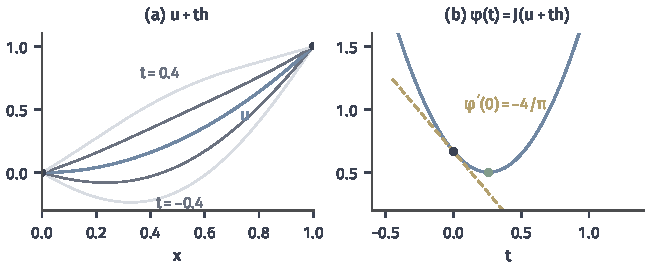
\includegraphics[width=110mm]{figures/03-optimization-evolution-and-signals/01-optimization/matplotlib/c9-perturbation-family/figure.pdf}
  \caption{沿一个方向扰动整条函数。(a)~$u(x)=x^2$（蓝）加上$t\sin(\pi x)$，$t=\pm0.2,\pm0.4$（灰），端点保持在$(0,0)$与$(1,1)$；(b)~目标$J_0(u+th)=\frac23-\frac4\pi t+\frac{\pi^2}4t^2$作为$t$的一元函数，黑点处虚线切线的斜率$-4/\pi$即方向导数，绿点是这条直线上的最小点。}
  \label{fig:opt-fn-perturbation-family}
\end{figure}

\paragraph{参数到函数的映射}
非线性参数拟合中，候选写成$u_{\bm\theta}$，参数$\bm\theta\in\mathbb R^p$的变化先通过映射$\bm\theta\mapsto u_{\bm\theta}$产生函数扰动。沿参数方向$\bm\eta$求导时，候选沿曲线$t\mapsto u_{\bm\theta+t\bm\eta}$而不是直线移动；在下文Fréchet微分的链式法则条件下，参数梯度的第$k$个分量等于目标沿函数方向$\partial u_{\bm\theta}/\partial\theta_k$的响应。参数梯度只看得到这$p$个函数方向，因此它不等于函数空间中的梯度，两者的关系由参数化决定。

\paragraph{各方向都可导，仍不一定线性}
设候选只在二维族$u=a\varphi_1+b\varphi_2$中变化，$\varphi_1,\varphi_2$线性无关，目标经系数写成
\[
 J(a,b)=\frac{a^3}{a^2+b^2}\quad((a,b)\neq(0,0)),\qquad J(0,0)=0 .
\]
在原点沿非零方向$(h_1,h_2)$，$J(th_1,th_2)/t=h_1^3/(h_1^2+h_2^2)$与$t$无关，所以方向导数存在，等于$h_1^3/(h_1^2+h_2^2)$。它对方向不可加：沿$(1,0)$为$1$，沿$(0,1)$为$0$，沿$(1,1)$却是$1/2\neq1+0$。图~\ref{fig:opt-fn-nonlinear-directional}(b)在单位方向$(\cos\theta,\sin\theta)$上画出$\cos^3\theta$；任何线性函数在单位圆上都形如$c_1\cos\theta+c_2\sin\theta$，与$\cos^3\theta$在$\theta=0,\pi/2$处取值相同的只有$\cos\theta$，而两者在$\theta=\pi/4$处已经不同。逐方向求导得到的是一族互不协调的数，还不能像梯度那样统一运算。

\begin{figure}[!htb]
  \centering
  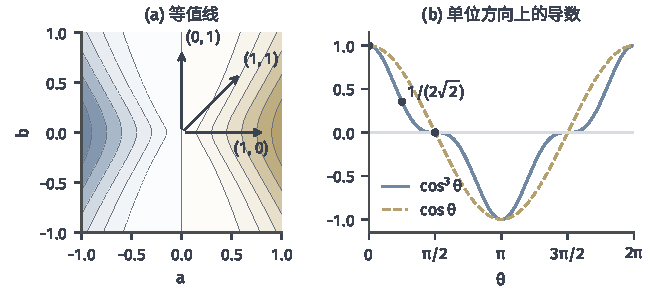
\includegraphics[width=110mm]{figures/03-optimization-evolution-and-signals/01-optimization/matplotlib/c9-nonlinear-directional/figure.pdf}
  \caption{方向导数都存在但不线性的例子$J(a,b)=a^3/(a^2+b^2)$。(a)~$J$的等值线（黄为正、蓝为负）与三个方向$(1,0)$、$(1,1)$、$(0,1)$；(b)~原点处沿单位方向$(\cos\theta,\sin\theta)$的方向导数$\cos^3\theta$（蓝），与线性函数$\cos\theta$（黄虚线）只在少数方向上相同。在$\theta=\pi/4$处前者为$1/(2\sqrt2)$，后者为$1/\sqrt2$。}
  \label{fig:opt-fn-nonlinear-directional}
\end{figure}

\subsection{Gâteaux微分}
\label{sec:opt-fn-gateaux}

上一个例子表明，要把方向响应当成一个对象来运算，还需要它们对方向线性。在函数空间里还要再加一条：响应不能被方向的范数无限放大，否则小扰动可能引起无界的变化。

\begin{definition}[Gâteaux微分]
\label{def:opt-fn-gateaux}
设$J$在$u$的某个开邻域内取有限值。若对每个$h\in X$方向导数$J'(u;h)$都存在，并且映射$h\mapsto J'(u;h)$是$X$上的有界线性泛函，则称$J$在$u$处Gâteaux可微，称这个泛函为$J$在$u$处的\term{Gâteaux微分}（Gâteaux derivative），记作$DJ(u)\in X^*$，$DJ(u)[h]=J'(u;h)$。
\end{definition}

先对每个固定方向取极限，再要求这些极限值组成有界线性泛函，这是本书的约定。有的文献只要求方向导数存在，或只要求线性，就称为Gâteaux可微；阅读时需要核对所用的定义。这里的$X^*$是$X$上全体有界线性泛函构成的对偶空间。

\paragraph{两个基本例子}
设$L:X\to\mathbb R$是有界线性泛函，则$(L(u+th)-Lu)/t=Lh$，所以$DL(u)=L$，与基点$u$无关。再设$X=H$是实Hilbert空间，$J(u)=\|u\|_H^2$。展开内积得
\[
 \frac{\|u+th\|_H^2-\|u\|_H^2}{t}=2\langle u,h\rangle_H+t\|h\|_H^2\longrightarrow2\langle u,h\rangle_H .
\]
映射$h\mapsto2\langle u,h\rangle_H$线性，由Cauchy--Schwarz不等式其范数不超过$2\|u\|_H$，所以$DJ(u)[h]=2\langle u,h\rangle_H$。同样的计算对~\eqref{eq:opt-fn-dirichlet-energy}给出$DJ_0(u)[h]=\int_0^1u'h'\,dx$，它满足$|DJ_0(u)[h]|\le\|u'\|_{L^2}\|h\|_{H^1}$。在这些例子里，方向响应都整理成了对偶空间中的一个元素。

\paragraph{逐方向极限还缺什么}
Gâteaux微分的定义只说：对每个固定的$h$，$t\to0$时误差相对于$t$趋于零。不同方向的趋零速度可以完全不同，定义对此不加控制。当扰动不沿任何固定直线、而是沿一条曲线趋于零时，线性近似可能失效；下一小节先给出这一要求，再用例子说明它确实更强。

\subsection{Fréchet微分}
\label{sec:opt-fn-frechet}

我们希望一个线性对象能同时预测所有足够小的扰动，而不仅是沿每条直线的扰动。这需要把误差相对于扰动的范数统一地控制住。

\begin{definition}[Fréchet微分]
\label{def:opt-fn-frechet}
设$J$在$u$的某个开邻域内取有限值。若存在有界线性泛函$A\in X^*$，使
\begin{equation}
 J(u+h)=J(u)+Ah+r(h),\qquad\lim_{\|h\|_X\to0}\frac{|r(h)|}{\|h\|_X}=0 ,
 \label{eq:opt-fn-frechet}
\end{equation}
则称$J$在$u$处Fréchet可微，$A$称为$J$在$u$处的\term{Fréchet微分}（Fréchet derivative）。余项条件常简写为$r(h)=o(\|h\|_X)$。
\end{definition}

余项条件中的极限对所有趋于零的$h$统一成立，与$h$沿什么路径趋于零无关。由此可以推出Gâteaux可微：固定$h\neq0$，令$t\to0$，则$\|th\|_X\to0$，
\[
 \Bigl|\frac{J(u+th)-J(u)}{t}-Ah\Bigr|=\frac{|r(th)|}{|t|}=\frac{|r(th)|}{\|th\|_X}\|h\|_X\longrightarrow0 .
\]
所以Fréchet可微时$J'(u;h)=Ah$对每个$h$成立，$A=DJ(u)$；两种微分若都存在则相同，以后统一记为$DJ(u)$。Fréchet可微还推出$J$在$u$处连续，因为$|J(u+h)-J(u)|\le\|A\|\|h\|_X+|r(h)|\to0$。

\paragraph{Gâteaux可微而非Fréchet可微}
在$\mathbb R^2$上取
\[
 f(a,b)=\frac{a^3b}{a^4+b^2}\quad((a,b)\neq(0,0)),\qquad f(0,0)=0 .
\]
由$a^4+b^2\ge2a^2|b|$得$|f(a,b)|\le|a|/2$，$f$在原点连续。沿方向$(h_1,h_2)$，$h_2\neq0$时$f(th_1,th_2)/t=t\,h_1^3h_2/(t^2h_1^4+h_2^2)\to0$，$h_2=0$时$f$恒为零，所以所有方向导数都是$0$：$f$在原点Gâteaux可微，微分为零泛函。然而沿抛物线$b=a^2$有$f(a,a^2)=a/2$；当$0<|a|\le1$时$\|(a,a^2)\|_2\le\sqrt2|a|$，余项比$|f(a,a^2)|/\|(a,a^2)\|_2\ge1/(2\sqrt2)$不趋于零，Fréchet条件~\eqref{eq:opt-fn-frechet}不成立。图~\ref{fig:opt-fn-gateaux-not-frechet}(b)显示了原因：沿每条固定射线，比值最终趋于零，但射线越贴近抛物线，开始下降的位置越靠近原点；抛物线从所有射线之间穿过，比值保持在$1/2$附近。

\begin{figure}[!htb]
  \centering
  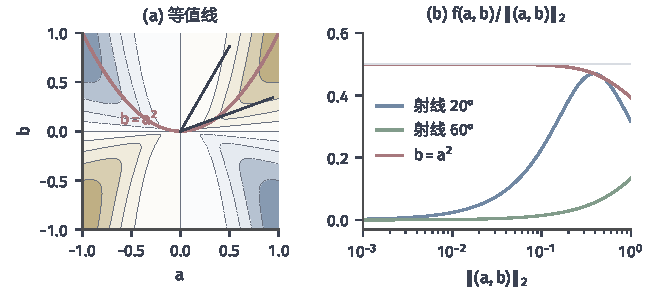
\includegraphics[width=110mm]{figures/03-optimization-evolution-and-signals/01-optimization/matplotlib/c9-gateaux-not-frechet/figure.pdf}
  \caption{Gâteaux可微但非Fréchet可微的$f(a,b)=a^3b/(a^4+b^2)$。(a)~等值线（黄为正、蓝为负）、两条过原点的射线（黑）与抛物线$b=a^2$（红）；(b)~比值$f/\|(a,b)\|_2$随到原点距离的变化（横轴对数）。沿$20^\circ$与$60^\circ$射线比值趋于零，沿抛物线趋于$1/2$。}
  \label{fig:opt-fn-gateaux-not-frechet}
\end{figure}

\paragraph{平方范数与平方误差}
对上一小节的两个例子保留完整的余项。平方范数满足$\|u+h\|_H^2=\|u\|_H^2+2\langle u,h\rangle_H+\|h\|_H^2$，余项$\|h\|_H^2$除以$\|h\|_H$后趋于零，所以它Fréchet可微。设$L\in X^*$，$y\in\mathbb R$，平方误差$E(u)=\frac12(Lu-y)^2$满足
\[
 E(u+h)=E(u)+(Lu-y)\,Lh+\tfrac12(Lh)^2,\qquad\tfrac12(Lh)^2\le\tfrac12\|L\|^2\|h\|_X^2 ,
\]
余项同样是$o(\|h\|_X)$，所以$DE(u)[h]=(Lu-y)Lh$。有限个这样的项相加时，余项相加仍是$o(\|h\|_X)$，这就是和法则；有限观测的平方误差$\frac12\sum_i(L_iu-y_i)^2$的微分是$\sum_i(L_iu-y_i)L_ih$。

\paragraph{链式法则}
复合映射的微分需要把内层映射也纳入同样的框架。设$Y$是赋范空间，映射$T:X\to Y$在$u$处Fréchet可微，指存在有界线性算子$DT(u):X\to Y$使$\|T(u+h)-T(u)-DT(u)h\|_Y=o(\|h\|_X)$。

\begin{theorem}[链式法则]
\label{thm:opt-fn-chain-rule}
设$T:X\to Y$在$u$处Fréchet可微，$G:Y\to\mathbb R\cup\{+\infty\}$在$T(u)$处Fréchet可微。则$G\circ T$在$u$处Fréchet可微，且
\[
 D(G\circ T)(u)[h]=DG(T(u))\bigl[DT(u)h\bigr] .
\]
\end{theorem}

\begin{proof}
记$k(h)=T(u+h)-T(u)$，$s(h)=k(h)-DT(u)h$，则$\|s(h)\|_Y=o(\|h\|_X)$，并且对足够小的$h$有$\|k(h)\|_Y\le(\|DT(u)\|+1)\|h\|_X$，所以$k(h)\to0$，$G$在$T(u+h)$处有限。由$G$的Fréchet可微性，$G(T(u+h))-G(T(u))=DG(T(u))[k(h)]+r_G(k(h))$，其中$r_G(k)=o(\|k\|_Y)$。代入$k(h)=DT(u)h+s(h)$，
\[
 \begin{aligned}
 &G(T(u+h))-G(T(u))-DG(T(u))[DT(u)h]\\
 &\qquad=DG(T(u))[s(h)]+r_G(k(h)) .
 \end{aligned}
\]
第一项的绝对值不超过$\|DG(T(u))\|\,\|s(h)\|_Y$，它是$o(\|h\|_X)$；第二项满足$|r_G(k(h))|\le\varepsilon\|k(h)\|_Y\le\varepsilon(\|DT(u)\|+1)\|h\|_X$，其中$\varepsilon$可随$h\to0$任意小。两项都是$o(\|h\|_X)$。
\end{proof}

最常用的情形是仿射内层映射$T(u)=Bu+b$，其中$B$是有界线性算子，此时$DT(u)=B$，余项$s\equiv0$。

\paragraph{积分目标与范数的选择}
对~\eqref{eq:opt-fn-dirichlet-energy}，$J_0(u+h)-J_0(u)-\int_0^1u'h'\,dx=\frac12\|h'\|_{L^2}^2\le\frac12\|h\|_{H^1}^2$，所以它在$H^1(0,1)$上Fréchet可微。一般的积分目标在把极限移入积分号之前，还要核验支配与可积条件，具体计算留到第~\ref{sec:opt-fn-integral}节。余项是否为$o(\|h\|_X)$取决于所选范数：同一个$J_0$在$L^2$范数下连有限邻域都没有。更换候选空间或范数时，Fréchet可微性必须重新检查。

\subsection{Hilbert梯度}
\label{sec:opt-fn-hilbert-gradient}

微分$DJ(u)$是对偶空间中的元素，它接收方向、返回数值；梯度下降需要的却是候选空间中的一个元素，以便写出$u-\eta\cdot(\text{某个方向})$。在Hilbert空间中，二者可以借内积互相转换。

\paragraph{由微分到梯度}
实Hilbert空间$H$上的每个有界线性泛函$\ell$都有唯一的$g\in H$使$\ell(h)=\langle g,h\rangle_H$对所有$h$成立，并且$\|\ell\|=\|g\|_H$。这就是Riesz表示定理，其证明及对偶空间的一般讨论见\BookChapterRef{chap:linear-functionals-operators}{卷二“线性泛函与线性算子”章}。把它用于$\ell=DJ(u)$，得到
\begin{equation}
 DJ(u)[h]=\langle\nabla_HJ(u),h\rangle_H\qquad\text{对所有}h\in H ,
 \label{eq:opt-fn-hilbert-gradient}
\end{equation}
称$\nabla_HJ(u)\in H$为$J$在$u$处关于内积$\langle\cdot,\cdot\rangle_H$的\term{梯度}（gradient）。由Cauchy--Schwarz不等式，在单位方向$\|h\|_H=1$中，$DJ(u)[h]\ge-\|\nabla_HJ(u)\|_H$，等号在$h=-\nabla_HJ(u)/\|\nabla_HJ(u)\|_H$时取到。下降最快的方向取决于用哪个内积计量“单位方向”。一般Banach空间中没有这样的表示，微分仍留在$X^*$中，不预设一个同空间的梯度。

\paragraph{同一个微分，不同的梯度}
在仿射函数$u(x)=a+bx$构成的二维空间上，固定目标$J(u)=(a^2+b^2)/2$。对方向$h=\alpha+\beta x$，$DJ(u)[h]=a\alpha+b\beta$，这个微分与内积无关。若按系数取内积$\langle u,h\rangle=a\alpha+b\beta$，梯度就是系数$(a,b)$对应的函数$a+bx$。若改用$[-1,1]$上的归一化$L^2$内积$\langle f,g\rangle=\frac12\int_{-1}^1fg\,dx$，则$\langle1,1\rangle=1$、$\langle1,x\rangle=0$、$\langle x,x\rangle=1/3$；寻找$c+dx$使$c\alpha+d\beta/3=a\alpha+b\beta$对所有$\alpha,\beta$成立，得$c=a$、$d=3b$，梯度是$a+3bx$。目标的微分没有改变，改变的只是用哪个元素代表它。若改动目标中观测的权重或能量的权重，改变的才是优化问题本身。

\paragraph{$L^2$梯度与$H^1$梯度}
同样的现象在无限维中有更直观的后果。在$H_0^1(0,1)$上考虑微分$\ell(h)=\int_0^1rh\,dx$，例如它是$J(u)=\frac12\int_0^1(u-g)^2dx$在$u-g=r$处的微分。若用$L^2$内积，梯度就是$r$。若用$H^1$内积$\langle w,h\rangle_{H^1}=\int_0^1(wh+w'h')\,dx$，取$r=\sum_kr_k\sin(k\pi x)$为有限正弦和，令
\[
 w=\sum_k\frac{r_k}{1+k^2\pi^2}\sin(k\pi x) .
\]
$w$光滑、两端为零，并满足$w-w''=r$。对任意$h\in H_0^1(0,1)$分部积分，边界项因$h(0)=h(1)=0$而消失，$\int_0^1(wh+w'h')\,dx=\int_0^1(w-w'')h\,dx=\int_0^1rh\,dx$，所以$w$就是$H^1$梯度。第$k$个频率被除以$1+k^2\pi^2$：图~\ref{fig:opt-fn-l2-h1-gradient}取$r=\sin(\pi x)+0.5\sin(15\pi x)$，高频成分相对低频的比例从$0.5$降到约$0.0024$。用$H^1$梯度作下降步，每一步加到候选上的修正更光滑。离散的梯度型更新沿用第~\ref{chap:opt-smooth}章的算法，连续时间的梯度流留给第~\ref{part:dynamical-systems-control-and-decision}部分。反过来也要注意，$L^2$梯度并不总在候选空间中：$DJ_0(u)[h]=\int u'h'$要写成$\int gh$，需要$u$有平方可积的二阶导数，此时$g=-u''$。

\begin{figure}[!htb]
  \centering
  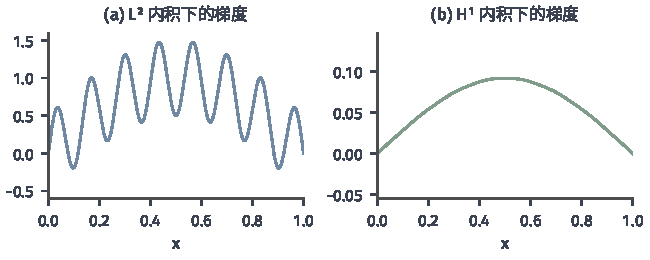
\includegraphics[width=110mm]{figures/03-optimization-evolution-and-signals/01-optimization/matplotlib/c9-l2-h1-gradient/figure.pdf}
  \caption{同一个微分$h\mapsto\int_0^1rh\,dx$在两种内积下的梯度。(a)~$L^2$梯度$r=\sin(\pi x)+0.5\sin(15\pi x)$；(b)~$H_0^1(0,1)$上$H^1$内积下的梯度$w=\sin(\pi x)/(1+\pi^2)+0.5\sin(15\pi x)/(1+225\pi^2)$，高频成分几乎被抹平。两图纵轴尺度不同。}
  \label{fig:opt-fn-l2-h1-gradient}
\end{figure}

% 第9章第2节：泛函的最优条件（无约束一阶条件、约束一阶条件、二阶条件）。

\section{泛函的最优条件}
\label{sec:opt-fn-optimality}

上一节只回答了“扰动之后目标怎样变化”。现在假定候选函数与所需微分都已给定，反过来问：若$u^\star$是最小点，这些变化必须满足什么条件？必要条件按允许的扰动方向逐一建立，充分条件则要求额外的结构。有限维中的同类结论见第~\ref{chap:optimization}章；本节说明哪些论证可以照搬，哪些在无限维中需要加强。

\subsection{无约束一阶条件}
\label{sec:opt-fn-unconstrained-first}

最小点附近，沿任何一条直线看过去，目标都不能下降。这一观察把函数空间中的问题化为一元函数的极值问题。

\begin{theorem}[一阶必要条件]
\label{thm:opt-fn-first-order-necessary}
设$J$在$u^\star$的某个开邻域$U$内取有限值，$u^\star$是$J$的局部最小点，即$J(u^\star)\le J(u)$对$U$中所有$u$成立。若$J$在$u^\star$处Gâteaux可微，则
\[
 DJ(u^\star)[h]=0\qquad\text{对所有}h\in X .
\]
在Hilbert空间中，这等价于$\nabla_HJ(u^\star)=0$。
\end{theorem}

\begin{proof}
固定$h$，令$\varphi(t)=J(u^\star+th)$。$|t|$足够小时$u^\star+th\in U$，所以$\varphi(t)\ge\varphi(0)$。$t>0$时差商$(\varphi(t)-\varphi(0))/t\ge0$，$t<0$时差商$\le0$；两侧极限都等于$DJ(u^\star)[h]$，故它既非负又非正，只能为零。
\end{proof}

证明只比较了$h$与$-h$两个方向上的一维变化，没有用到微分的线性。定理的前提是最小点存在；它只是筛选候选的条件，不能说明满足$DJ(u)=0$的$u$是最小点，也不能说明这样的$u$存在。

\paragraph{凸性给出充分性}
对凸目标，零微分已经足够。设$X$中的凸集$K$上$J$取有限值且凸，即对$u,v\in K$、$t\in[0,1]$有$J(u+t(v-u))\le(1-t)J(u)+tJ(v)$；凸函数及其一阶刻画的有限维版本见第~\ref{chap:optimization}章。若$J$在$K$的内点$u$处Gâteaux可微，则对每个$v\in K$，
\[
 \frac{J(u+t(v-u))-J(u)}t\le J(v)-J(u),\qquad0<t\le1 ;
\]
令$t\to0^+$，左边趋于$DJ(u)[v-u]$，得到一阶支撑不等式
\begin{equation}
 J(v)\ge J(u)+DJ(u)[v-u]\qquad\text{对所有}v\in K .
 \label{eq:opt-fn-convex-support}
\end{equation}
若$DJ(u^\star)=0$，则$J(v)\ge J(u^\star)$对所有$v\in K$成立，$u^\star$是$K$上的全局最小点。

\paragraph{驻点可以不是最小点}
在$X=L^2(0,1)$上取$J_1(u)=-\bigl(\int_0^1u\,dx\bigr)^2$与$J_2(u)=\bigl(\int_0^1u\,dx\bigr)^3$。两者在$u=0$处的微分都是零：$J_1(th)=-t^2(\int h)^2$，$J_2(th)=t^3(\int h)^3$，除以$t$后都趋于零。限制到常函数$u\equiv c$上，它们分别是$-c^2$和$c^3$，零点分别是最大点和没有极值的点。零微分方程“解出来了”并不意味着找到了最小点，从必要条件到充分条件需要凸性或下面的二阶条件这样的额外结构。

\subsection{约束一阶条件}
\label{sec:opt-fn-constrained-first}

候选受约束时，$u^\star+th$可能离开可行集，上一小节的双向比较不再可用。我们先看哪些扰动保持可行，再在这些方向上重复同样的论证。

\paragraph{仿射约束：在方向空间上为零}
章首的固定端点问题中，可行集$C=\{u\in H^1(0,1):u(0)=0,u(1)=1\}$是仿射集：任取$u_0\in C$（例如$u_0(x)=x$），则$C=u_0+V$，其中$V=\{h\in H^1(0,1):h(0)=h(1)=0\}=H_0^1(0,1)$。对$u\in C$与$h\in V$，$u+th$对所有实数$t$都可行，可以作正负两个方向的扰动。均值约束$\int_0^1u\,dx=m$同样给出仿射集，方向空间是$\{h:\int_0^1h\,dx=0\}$。

\begin{theorem}[仿射约束下的一阶必要条件]
\label{thm:opt-fn-affine-first-order}
设$C=u_0+V$，$V$是$X$的线性子空间，$J$在$u^\star\in C$的某个开邻域内取有限值且在$u^\star$处Gâteaux可微。若$u^\star$是$J$在$C$上的局部最小点，则$DJ(u^\star)[h]=0$对所有$h\in V$成立。
\end{theorem}

证明与定理~\ref{thm:opt-fn-first-order-necessary}相同，只是$h$限于$V$。结论只约束微分在$V$上的作用，不要求整个微分为零。固定端点问题中，最优点满足$\int_0^1u^{\star\prime}h'\,dx=0$对所有$h\in H_0^1(0,1)$成立，而不是对所有$h\in H^1(0,1)$：取$h\equiv1$时$\int u^{\star\prime}\cdot0=0$自然成立，取$h(x)=x$则一般不为零，这个方向会破坏端点条件，不在允许之列。

\paragraph{凸约束：变分不等式}
可行集是凸集但不是仿射集时，只能沿指向集合内部的线段移动。设$C$凸，$u^\star\in C$，$v\in C$，则线段$u^\star+t(v-u^\star)$，$t\in[0,1]$，留在$C$中。

\begin{theorem}[凸约束下的一阶条件]
\label{thm:opt-fn-variational-inequality}
设$C\subseteq X$凸，$J$在$u^\star\in C$的某个开邻域内取有限值且在$u^\star$处Gâteaux可微。
\begin{enumerate}
 \item 若$u^\star$是$J$在$C$上的局部最小点，则
 \begin{equation}
  DJ(u^\star)[v-u^\star]\ge0\qquad\text{对所有}v\in C .
  \label{eq:opt-fn-variational-inequality}
 \end{equation}
 \item 若$J$在一个包含$C$的凸集上凸，则~\eqref{eq:opt-fn-variational-inequality}推出$u^\star$是$J$在$C$上的全局最小点。
\end{enumerate}
\end{theorem}

\begin{proof}
(1) 令$\varphi(t)=J(u^\star+t(v-u^\star))$。$t>0$足够小时$\varphi(t)\ge\varphi(0)$，所以单侧差商非负，其极限$DJ(u^\star)[v-u^\star]\ge0$。(2) 由支撑不等式~\eqref{eq:opt-fn-convex-support}，$J(v)\ge J(u^\star)+DJ(u^\star)[v-u^\star]\ge J(u^\star)$。
\end{proof}

形如~\eqref{eq:opt-fn-variational-inequality}的条件称为\term{变分不等式}（variational inequality）。它只要求微分在指向可行集的方向上非负，边界上的最小点不必使整个空间的梯度为零。

\begin{example}[非负约束下的最近函数]
\label{ex:opt-fn-positivity}
在$X=L^2(0,1)$中取$g(x)=\sin(2\pi x)$，在$C=\{u\in L^2(0,1):u\ge0\text{ 几乎处处}\}$上最小化$J(u)=\frac12\int_0^1(u-g)^2dx$。$C$凸，$J$凸且$\nabla_{L^2}J(u)=u-g$。候选$u^\star=\max(g,0)$满足变分不等式：$u^\star-g=\max(-g,0)$只在$u^\star=0$的地方不为零，于是对任意$v\in C$，
\[
 \int_0^1(u^\star-g)(v-u^\star)\,dx=\int_{\{g<0\}}(-g)\,v\,dx\ge0 .
\]
由定理~\ref{thm:opt-fn-variational-inequality}(2)，$u^\star$是全局最小点，最小值为$\frac12\int_{\{g<0\}}g^2dx=1/8$。图~\ref{fig:opt-fn-positivity-vi}中，梯度$u^\star-g$（黄）在后半区间明显不为零，它“想把”$u$往下推，但那里$u^\star$已贴着约束$u\ge0$，任何可行方向$v-u^\star$在该处都非负，内积因而非负。
\end{example}

\begin{figure}[!htb]
  \centering
  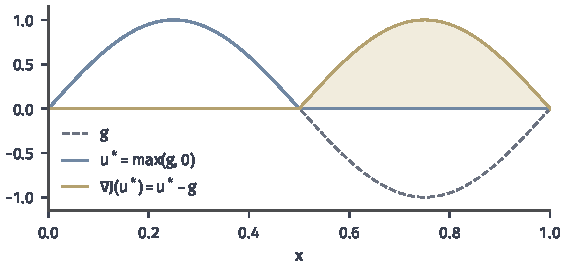
\includegraphics[width=96mm]{figures/03-optimization-evolution-and-signals/01-optimization/matplotlib/c9-positivity-vi/figure.pdf}
  \caption{非负约束下的最优函数。灰色虚线为$g(x)=\sin(2\pi x)$，蓝线为最优解$u^\star=\max(g,0)$（图中记作$u^*$），黄线及浅黄区域为梯度$u^\star-g=\max(-g,0)$。梯度只在$u^\star=0$处非零，并且指向约束之外，满足变分不等式而不等于零。}
  \label{fig:opt-fn-positivity-vi}
\end{figure}

\paragraph{非凸约束}
若$C$不凸，$u^\star$与$v\in C$之间的线段可能离开$C$，变分不等式的推导失效。这时需要重新描述可行方向，例如沿留在$C$中的曲线$t\mapsto c(t)$求导；等式约束$\|u\|_H=1$这样的球面就属于此类，其处理方式与第~\ref{chap:constrained-optimization}章中有限维的切方向和KKT条件相同，本章不再展开。

\subsection{二阶条件}
\label{sec:opt-fn-second-order}

一阶条件无法区分最小点与最大点。和有限维一样，下一步看二阶项；无限维中的新问题在于“正定”需要一个统一的下界。

\paragraph{二阶展开}
设$J$在$u$的开邻域内有限，若存在有界线性泛函$DJ(u)$与有界对称双线性形式$D^2J(u):X\times X\to\mathbb R$，使
\begin{equation}
 J(u+h)=J(u)+DJ(u)[h]+\tfrac12D^2J(u)[h,h]+o(\|h\|_X^2) ,
 \label{eq:opt-fn-second-expansion}
\end{equation}
就说$J$在$u$处有二阶展开。例如平方误差$E(u)=\frac12(Lu-y)^2$的展开是精确的，$D^2E(u)[h,h]=(Lh)^2$；$J_0$的二阶项是$\int_0^1h'^2dx$。

\begin{theorem}[二阶条件]
\label{thm:opt-fn-second-order}
设$C=u^\star+V$，$V$为线性子空间（$V=X$即无约束情形），$J$在$u^\star$处有二阶展开~\eqref{eq:opt-fn-second-expansion}。
\begin{enumerate}
 \item 若$u^\star$是$J$在$C$上的局部最小点，则对所有$h\in V$，都有$DJ(u^\star)[h]=0$，并且$D^2J(u^\star)[h,h]\ge0$。
 \item 若对所有$h\in V$都有$DJ(u^\star)[h]=0$，并且存在常数$c>0$，使所有$h\in V$满足$D^2J(u^\star)[h,h]\ge c\|h\|_X^2$，则存在$\rho>0$，使$h\in V$、$\|h\|_X<\rho$时
 \[
  J(u^\star+h)\ge J(u^\star)+\tfrac c4\|h\|_X^2 .
 \]
 特别地，$u^\star$是$C$上的严格局部最小点。
\end{enumerate}
\end{theorem}

\begin{proof}
(1) 一阶部分即定理~\ref{thm:opt-fn-affine-first-order}。固定$h\in V$，$t\to0$时$0\le J(u^\star+th)-J(u^\star)=\frac{t^2}2D^2J(u^\star)[h,h]+o(t^2)$，两边除以$t^2$再取极限即得。(2) 取$\rho$使$\|h\|_X<\rho$时余项绝对值不超过$\frac c4\|h\|_X^2$，则$J(u^\star+h)-J(u^\star)\ge\frac c2\|h\|_X^2-\frac c4\|h\|_X^2$。
\end{proof}

必要条件只要求二阶项半正定，充分条件要求一致的正下界$c$。一般非线性约束下的二阶判别还涉及约束本身的曲率与临界方向，不能只看目标的二阶项，本节不讨论。

\paragraph{每个方向为正，仍可能不是最小点}
有限维中，二次型在每个非零方向上为正就推出存在共同的$c>0$，因为单位球面是紧集。无限维中单位球面不紧，这一步失败。在$\ell^2$上取
\[
 J(\bm x)=\sum_{k=1}^\infty\frac{x_k^2}k-\sum_{k=1}^\infty x_k^4 .
\]
由$\sum_kx_k^4\le(\sum_kx_k^2)^2=\|\bm x\|_2^4$，第二项是$o(\|\bm x\|_2^2)$，所以$J$在原点的二阶展开为$DJ(0)=0$、$D^2J(0)[\bm h,\bm h]=2\sum_kh_k^2/k$，对每个$\bm h\neq0$都为正。但没有共同的$c$：沿第$k$个坐标方向$\bm e_k$，$D^2J(0)[\bm e_k,\bm e_k]=2/k\to0$。原点也确实不是局部最小点：$J(t\bm e_k)=t^2/k-t^4$在$t>1/\sqrt k$时为负，而$1/\sqrt k\to0$，原点的任意小邻域里都有使$J<0=J(0)$的点。图~\ref{fig:opt-fn-no-uniform-curvature}画出这些截线：每条在原点附近都向上弯，但弯曲越来越平，越过零点的位置越来越靠近原点。

\begin{figure}[!htb]
  \centering
  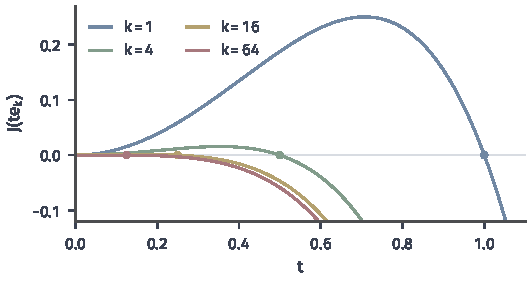
\includegraphics[width=90mm]{figures/03-optimization-evolution-and-signals/01-optimization/matplotlib/c9-no-uniform-curvature/figure.pdf}
  \caption{二阶项逐方向为正但没有一致下界。$\ell^2$上$J(\bm x)=\sum_kx_k^2/k-\sum_kx_k^4$沿坐标方向的截线$J(t\bm e_k)=t^2/k-t^4$，$k=1,4,16,64$；圆点标出零点$t=1/\sqrt k$。原点处每条截线的二阶导数$2/k$都为正，零点却随$k$增大逼近原点。}
  \label{fig:opt-fn-no-uniform-curvature}
\end{figure}

% 第9章第3节：积分泛函的变分（一阶变分的计算、Euler--Lagrange方程、边界条件）。

\section{积分泛函的变分}
\label{sec:opt-fn-integral}

最常见的目标泛函是对局部代价的积分：每个位置$x$上，代价由$x$、函数值$u(x)$和导数$u'(x)$决定，再沿整个区间累加。本节固定这类目标，先计算它的一阶变化，再分别用内部扰动和边界扰动从最优条件中提取两类信息：区间内部的微分方程与边界上的条件。

\subsection{一阶变分的计算}
\label{sec:opt-fn-first-variation}

\paragraph{一维积分泛函}
设$F(x,s,p)$是定义在$[a,b]\times\mathbb R\times\mathbb R$上的函数，称为密度，目标为
\begin{equation}
 J(u)=\int_a^bF\bigl(x,u(x),u'(x)\bigr)\,dx .
 \label{eq:opt-fn-integral-functional}
\end{equation}
用$F_s$、$F_p$表示$F$对第二、第三个变量的偏导数；沿候选$u$求值时，习惯上写成$F_u=F_s(x,u,u')$、$F_{u'}=F_p(x,u,u')$。记号$F_{u'}$表示“对导数所在的那个变量求偏导”，不是对$u'$这个函数求导。

\begin{theorem}[积分泛函的方向导数]
\label{thm:opt-fn-first-variation}
设$F$对$(s,p)$连续可微，$u,h$使$J(u+th)$对$|t|\le t_0$有限，并存在可积函数$m$，使对几乎所有$x$及所有$|\tau|\le t_0$，
\begin{equation}
 \bigl|F_s(x,u+\tau h,u'+\tau h')\,h+F_p(x,u+\tau h,u'+\tau h')\,h'\bigr|\le m(x) .
 \label{eq:opt-fn-domination}
\end{equation}
则
\begin{equation}
 J'(u;h)=\int_a^b\bigl(F_u\,h+F_{u'}\,h'\bigr)\,dx .
 \label{eq:opt-fn-first-variation}
\end{equation}
\end{theorem}

\begin{proof}
固定$x$，$\tau\mapsto F(x,u+\tau h,u'+\tau h')$连续可微，由中值定理，对$0<|t|\le t_0$，差商$\bigl(F(x,u+th,u'+th')-F(x,u,u')\bigr)/t$等于~\eqref{eq:opt-fn-domination}左侧绝对值号内的表达式在某个$\tau\in(0,t)$（或$(t,0)$）处的值，因此被$m(x)$控制；$t\to0$时它逐点趋于$F_uh+F_{u'}h'$。由控制收敛定理，积分与极限可以交换。
\end{proof}

若$F$对$(s,p)$连续可微且对$x$连续，$u,h\in C^1[a,b]$，则$(x,\tau)$在紧集$[a,b]\times[-t_0,t_0]$上，~\eqref{eq:opt-fn-domination}左侧连续因而有界，支配条件自动成立。对一般的Sobolev候选，支配需要从$F$的增长条件中逐项核验。还要注意，~\eqref{eq:opt-fn-first-variation}只计算了目标的响应，它是否在所有方向上线性有界、是否为零，是后面最优条件要讨论的事。

\paragraph{两个密度}
导数平方能量$F=\frac12p^2$给出$J_0'(u;h)=\int_a^bu'h'\,dx$，与上一节一致。弧长$F=\sqrt{1+p^2}$度量曲线$x\mapsto(x,u(x))$的长度，$F_p=p/\sqrt{1+p^2}$，于是$\ell'(u;h)=\int_a^bu'h'/\sqrt{1+u'^2}\,dx$；$|F_p|\le1$，只要$h'$可积，支配条件就成立。

\paragraph{多元区域与多分量场}
设$\Omega\subset\mathbb R^d$为有界Lipschitz区域，目标为$J(u)=\int_\Omega F(x,u,\nabla u)\,dx$。对标量场$u:\Omega\to\mathbb R$，$\nabla u(x)\in\mathbb R^d$，密度对第三个变量的偏导$F_{\nabla u}$也是$\mathbb R^d$中的向量。对多分量场$u:\Omega\to\mathbb R^m$，$\nabla u(x)$是$m\times d$矩阵，第$(i,j)$个元素为$\partial_ju_i$；$F_u\in\mathbb R^m$，$F_{\nabla u}$是同形状的$m\times d$矩阵。在与定理~\ref{thm:opt-fn-first-variation}相同的可微与支配条件下，
\[
 J'(u;h)=\int_\Omega\bigl(F_u\cdot h+F_{\nabla u}:\nabla h\bigr)\,dx,\qquad A:B=\sum_{i,j}A_{i,j}B_{i,j} .
\]
标量情形中$F_{\nabla u}:\nabla h$就是内积$F_{\nabla u}\cdot\nabla h$。逐项核对类型可以避免把矩阵与向量混在一起。这样的形式计算还不是任意Sobolev泛函可微性的证明；支配条件需要对具体密度验证。

\paragraph{平滑的导数幅度}
导数平方能量对大斜率惩罚很重。若只想惩罚导数的大小，可以用$\|\nabla u\|$代替$\|\nabla u\|^2$，但它在零梯度处不可微。取$\varepsilon>0$，在$H^1(\Omega)$上考虑
\begin{equation}
 J_\varepsilon(u)=\int_\Omega\psi_\varepsilon(\nabla u)\,dx,\qquad\psi_\varepsilon(\bm p)=\sqrt{\|\bm p\|_2^2+\varepsilon^2} .
 \label{eq:opt-fn-smoothed-tv}
\end{equation}
由$\psi_\varepsilon(\bm p)\le\|\bm p\|_2+\varepsilon$，$J_\varepsilon$在有界区域上处处有限。密度的梯度与Hessian为
\[
 \nabla\psi_\varepsilon(\bm p)=\frac{\bm p}{\sqrt{\|\bm p\|_2^2+\varepsilon^2}},\qquad\nabla^2\psi_\varepsilon(\bm p)=\frac1{\psi_\varepsilon(\bm p)}\Bigl(\bm I-\frac{\bm p\bm p^\top}{\psi_\varepsilon(\bm p)^2}\Bigr) .
\]
前者的范数不超过$1$；后者的特征值在$0$与$1/\psi_\varepsilon(\bm p)\le1/\varepsilon$之间，所以$\nabla\psi_\varepsilon$是$1/\varepsilon$-Lipschitz的。由此
\[
 \bigl|\psi_\varepsilon(\bm p+\bm q)-\psi_\varepsilon(\bm p)-\nabla\psi_\varepsilon(\bm p)\cdot\bm q\bigr|\le\frac{\|\bm q\|_2^2}{2\varepsilon} .
\]
取$\bm p=\nabla u(x)$、$\bm q=\nabla h(x)$并积分，
\[
 \Bigl|J_\varepsilon(u+h)-J_\varepsilon(u)-\int_\Omega\frac{\nabla u\cdot\nabla h}{\sqrt{\|\nabla u\|_2^2+\varepsilon^2}}\,dx\Bigr|\le\frac{\|\nabla h\|_{L^2}^2}{2\varepsilon}\le\frac{\|h\|_{H^1}^2}{2\varepsilon} .
\]
中间的积分对$h$线性，并且不超过$\int_\Omega\|\nabla h\|_2\le|\Omega|^{1/2}\|h\|_{H^1}$，所以$J_\varepsilon$在$H^1(\Omega)$的每一点Fréchet可微。这里有界的密度导数提供了支配，$1/\varepsilon$的Lipschitz界控制了二阶余项。$\varepsilon=0$时$\psi_0(\bm p)=\|\bm p\|_2$在$\bm p=0$处有尖点（图~\ref{fig:opt-fn-smoothed-abs}），梯度为零的区域上需要改用第~\ref{chap:opt-nonsmooth}章的次梯度，上面的光滑计算不能沿用。一维时$\varepsilon=1$的$J_1$恰好是弧长。

\begin{figure}[!htb]
  \centering
  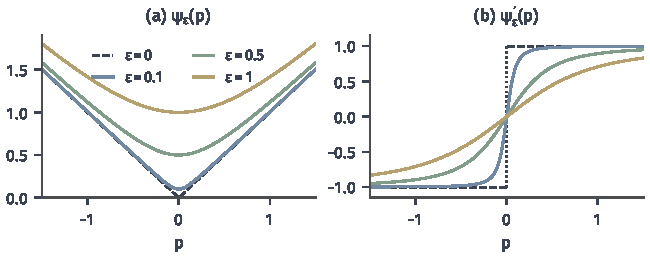
\includegraphics[width=110mm]{figures/03-optimization-evolution-and-signals/01-optimization/matplotlib/c9-smoothed-abs/figure.pdf}
  \caption{一维的平滑导数幅度密度。(a)~$\psi_\varepsilon(p)=\sqrt{p^2+\varepsilon^2}$，$\varepsilon=0.1,0.5,1$，黑色虚线为$\varepsilon=0$时的$|p|$；(b)~导数$p/\sqrt{p^2+\varepsilon^2}$，取值在$(-1,1)$内，在$p=0$处斜率最大，为$1/\varepsilon$。$\varepsilon\to0$时导数趋于在零点跳跃的符号函数（黑色虚线）。}
  \label{fig:opt-fn-smoothed-abs}
\end{figure}

\subsection{Euler--Lagrange方程}
\label{sec:opt-fn-euler-lagrange}

一阶变分~\eqref{eq:opt-fn-first-variation}同时含有$h$和$h'$。若最优条件要求它对许多$h$为零，我们希望把$h'$转移成$h$，得到一个只乘以$h$的积分，再由$h$的任意性推出被积函数为零。分部积分完成转移，代价是出现边界项；先选在边界附近为零的扰动，让边界项消失。

\paragraph{变分基本引理}
用$C_c^\infty(a,b)$表示在$(a,b)$内某个闭子区间外恒为零的光滑函数，称为测试函数。

\begin{lemma}[变分基本引理]
\label{lem:opt-fn-fundamental}
设$w$在$(a,b)$上连续，且$\int_a^bw\varphi\,dx=0$对所有$\varphi\in C_c^\infty(a,b)$成立，则$w\equiv0$。
\end{lemma}

\begin{proof}
若某点$x_0$处$w(x_0)>0$，由连续性存在$\delta>0$使$w>w(x_0)/2$在$(x_0-\delta,x_0+\delta)\subset(a,b)$上成立。取一个在此区间外为零、在区间内为正的光滑凸起函数$\varphi$，则$\int w\varphi>0$，矛盾。$w(x_0)<0$同理。
\end{proof}

$w$只局部可积时，结论改为$w=0$几乎处处，这正是卷二中弱导数唯一性所依据的事实。下面的推导在内部只用测试函数，所以引理适用于约束为固定端点、零扰动迹或其他只限制边界的情形。

\paragraph{一维方程}
设$u^\star$是$J$在某个可行集上的局部最小点，可行集允许所有$u^\star+t\varphi$（$\varphi\in C_c^\infty(a,b)$，$|t|$小），并且~\eqref{eq:opt-fn-first-variation}对这些方向成立。由定理~\ref{thm:opt-fn-first-order-necessary}的论证，
\begin{equation}
 \int_a^b\bigl(F_u\,\varphi+F_{u'}\,\varphi'\bigr)\,dx=0\qquad\text{对所有}\varphi\in C_c^\infty(a,b) .
 \label{eq:opt-fn-weak-el}
\end{equation}
若$x\mapsto F_{u'}(x,u^\star,u^{\star\prime})$连续可微（例如$u^\star\in C^2$且$F$二次连续可微），分部积分，边界项因$\varphi(a)=\varphi(b)=0$消失，得$\int_a^b\bigl(F_u-\frac{d}{dx}F_{u'}\bigr)\varphi\,dx=0$。由引理~\ref{lem:opt-fn-fundamental}，
\begin{equation}
 F_u-\frac{d}{dx}F_{u'}=0\qquad\text{在}(a,b)\text{上} .
 \label{eq:opt-fn-el}
\end{equation}
称为\term{Euler--Lagrange方程}（Euler--Lagrange equation）。没有这样的光滑性时，保留积分形式~\eqref{eq:opt-fn-weak-el}：它恰好说明$F_{u'}$的弱导数存在并等于$F_u$，因为弱导数的定义正是$\int F_{u'}\varphi'=-\int F_u\varphi$对一切测试函数成立。这称为方程的弱形式，只对合法的测试函数断言等式。

\paragraph{多元方程}
在有界Lipschitz区域$\Omega\subset\mathbb R^d$上，用$C_c^\infty(\Omega)$中的测试函数和散度定理代替一维分部积分，相同的论证在足够光滑时给出
\[
 F_u-\operatorname{div}F_{\nabla u}=0\qquad\text{在}\Omega\text{内},
\]
其中对多分量场按分量理解：第$i$个方程为$(F_u)_i-\sum_j\partial_j(F_{\nabla u})_{i,j}=0$。光滑性不足时同样保留弱形式$\int_\Omega(F_u\cdot\varphi+F_{\nabla u}:\nabla\varphi)\,dx=0$。

\paragraph{候选方程与最优性论证}
对固定端点的导数平方能量~\eqref{eq:opt-fn-dirichlet-energy}，$F_u=0$、$F_{u'}=u'$，方程~\eqref{eq:opt-fn-el}化为$u''=0$，满足$u(0)=0,u(1)=1$的解是$u^\star(x)=x$。这一步只得到了候选，最优性另需论证。任取$v\in C$，令$h=v-u^\star\in H_0^1(0,1)$，则
\[
 \begin{aligned}
 J_0(v)&=J_0(u^\star)+\int_0^1h'\,dx+\frac12\int_0^1h'^2\,dx\\
 &=J_0(u^\star)+\bigl[h\bigr]_0^1+\frac12\int_0^1h'^2\,dx=\frac12+\frac12\int_0^1h'^2\,dx .
 \end{aligned}
\]
所以$J_0(v)\ge J_0(u^\star)=1/2$，等号当且仅当$h'=0$几乎处处，结合$h(0)=0$即$h=0$。$u^\star$是唯一的最小点。这里起作用的是平方差展开，也就是$J_0$的凸性，而不是“解出了方程”。

\paragraph{能量与长度}
图~\ref{fig:opt-fn-fixed-endpoint-candidates}比较了几条固定端点的曲线。直线$x$的能量$1/2$与长度$\sqrt2\approx1.414$都最小；弧长的Euler--Lagrange方程$\frac{d}{dx}\bigl(u'/\sqrt{1+u'^2}\bigr)=0$推出$u'$为常数，同样给出直线。最优性仍要单独论证：$\sqrt{1+p^2}$是凸函数，弧长因而是凸泛函，由支撑不等式~\eqref{eq:opt-fn-convex-support}，$\ell(v)\ge\ell(x)+\int_0^1\frac{h'}{\sqrt2}\,dx=\ell(x)$，其中$h=v-x$两端为零。两个目标对其他曲线的评判却不同：$\sqrt x$是$x^2$关于对角线的镜像，长度相同，但它在原点处斜率无界，$\int_0^1u'^2dx=\int_0^1\frac{dx}{4x}=+\infty$，导数平方能量把它排除在$H^1$之外。

\begin{figure}[!htb]
  \centering
  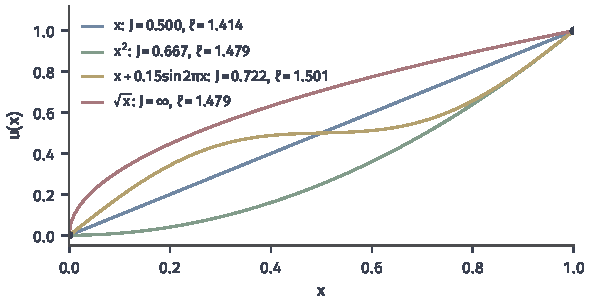
\includegraphics[width=100mm]{figures/03-optimization-evolution-and-signals/01-optimization/matplotlib/c9-fixed-endpoint-candidates/figure.pdf}
  \caption{连接$(0,0)$与$(1,1)$的四条曲线及其导数平方能量$J=\frac12\int_0^1u'^2dx$和弧长$\ell=\int_0^1\sqrt{1+u'^2}\,dx$。直线$x$同时使两者最小（$J=1/2$，$\ell=\sqrt2$）；$x^2$与$\sqrt x$互为镜像，长度同为约$1.479$，后者的能量却是无穷大。}
  \label{fig:opt-fn-fixed-endpoint-candidates}
\end{figure}

\paragraph{非二次能量的内部方程}
对~\eqref{eq:opt-fn-smoothed-tv}，$F_u=0$，$F_{\nabla u}=\nabla u/\sqrt{\|\nabla u\|_2^2+\varepsilon^2}$，内部方程是
\[
 -\operatorname{div}\frac{\nabla u}{\sqrt{\|\nabla u\|_2^2+\varepsilon^2}}=0 .
\]
一维时它说明$u'/\sqrt{u'^2+\varepsilon^2}$为常数，从而$u'$为常数，固定端点下又得到直线。多维时这是一个非线性方程，其解的存在性与正则性不能由这里的推导得到；第~\ref{sec:opt-fn-existence}节将看到，即使存在性论证本身也需要额外的依据。具体方程的解理论由第~\ref{part:dynamical-systems-control-and-decision}部分继续处理。

\subsection{边界条件}
\label{sec:opt-fn-boundary}

上一小节有意让边界项消失。若可行集允许候选在边界上变化，最优条件就会对边界项提出要求；哪些边界扰动合法，由可行集决定。

\paragraph{一维的边界项}
保留分部积分的边界项，在~\eqref{eq:opt-fn-el}所需的光滑性下，
\begin{equation}
 J'(u;h)=\int_a^b\Bigl(F_u-\frac{d}{dx}F_{u'}\Bigr)h\,dx+\Bigl[F_{u'}\,h\Bigr]_a^b .
 \label{eq:opt-fn-boundary-term}
\end{equation}
设最优点$u^\star$只受左端条件$u(a)=\alpha$约束，右端自由。先用测试函数得到内部方程，~\eqref{eq:opt-fn-boundary-term}中的积分对所有合法$h$都消失；再取满足$h(a)=0$、$h(b)=1$的光滑$h$，剩下的边界项给出
\[
 F_{u'}\bigl(b,u^\star(b),u^{\star\prime}(b)\bigr)=0 .
\]
这个条件不是事先规定的，而是由最优性推出的，称为\term{自然边界条件}（natural boundary condition）。直接写进可行集的条件$u(a)=\alpha$则相应地称为\term{本质边界条件}（essential boundary condition）：那里扰动必须满足$h(a)=0$，边界项自动消失，不产生新的方程。

\begin{example}[固定端与自由端]
\label{ex:opt-fn-free-end}
在$[0,1]$上最小化$J(u)=\int_0^1\bigl(\tfrac12u'^2-u\bigr)\,dx$。$F_u=-1$，$F_{u'}=u'$，内部方程为$-u''=1$。两端固定为零时，解是$u=x(1-x)/2$，$J=-1/24$。只固定$u(0)=0$、右端自由时，自然边界条件为$u'(1)=0$，解是$u=x-x^2/2$，$J=-1/6$。两个问题的目标都是凸的，与上一小节相同的平方差展开说明这两个解分别是各自可行集上的唯一最小点。图~\ref{fig:opt-fn-boundary-conditions}中，右端自由的曲线以水平切线到达边界；可行集更大，最小值也更低。
\end{example}

\begin{figure}[!htb]
  \centering
  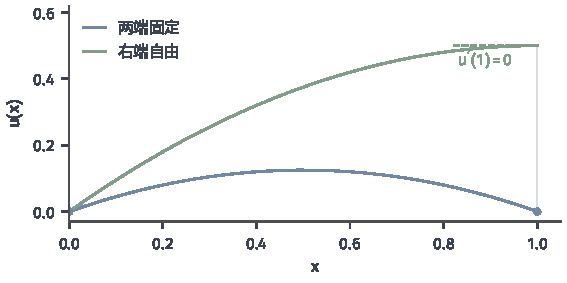
\includegraphics[width=96mm]{figures/03-optimization-evolution-and-signals/01-optimization/matplotlib/c9-boundary-conditions/figure.pdf}
  \caption{同一目标$J(u)=\int_0^1(\frac12u'^2-u)\,dx$在两种边界条件下的最优解。两端固定时（蓝）解为$x(1-x)/2$，$J=-1/24$；右端自由时（绿）解为$x-x^2/2$，在$x=1$处满足自然边界条件$u'(1)=0$，$J=-1/6$。}
  \label{fig:opt-fn-boundary-conditions}
\end{figure}

\paragraph{多元区域的边界}
在$\Omega$上用散度定理，足够光滑时
\[
 J'(u;h)=\int_\Omega\bigl(F_u-\operatorname{div}F_{\nabla u}\bigr)\cdot h\,dx+\int_{\partial\Omega}\bigl(F_{\nabla u}\bm n\bigr)\cdot h\,dS ,
\]
其中$\bm n$是单位外法向量；多分量情形$F_{\nabla u}\bm n$是$m\times d$矩阵乘以$d$维向量，得到$m$维的通量。若边界分为固定部分$\Gamma_D$与自由部分$\Gamma_N$，则$\Gamma_D$上扰动迹为零，$\Gamma_N$上允许任意的边界扰动，于是在$\Gamma_N$上得到$F_{\nabla u}\bm n=0$。若目标还含边界代价$\int_{\Gamma_N}G(x,u)\,dS$，它的一阶变化$\int_{\Gamma_N}G_u\cdot h\,dS$并入边界项，自然条件变为$F_{\nabla u}\bm n+G_u=0$。

\paragraph{梯度场拟合的边界含义}
第~\ref{chap:opt-function-fitting}章用闭子空间投影求得了梯度场拟合问题的解：给定向量场$v\in L^2(\Omega;\mathbb R^d)$，最小化$\frac12\int_\Omega\|\nabla u-v\|_2^2dx$，并由投影余项的正交性得到$\int_\Omega(\nabla u-v)\cdot\nabla h\,dx=0$。这正是密度$F=\frac12\|\nabla u-v\|_2^2$的一阶条件，$F_{\nabla u}=\nabla u-v$。足够光滑时，内部给出$\operatorname{div}(\nabla u-v)=0$；若边界自由，自然边界条件是
\[
 (\nabla u-v)\cdot\bm n=0\qquad\text{在}\partial\Omega\text{上} .
\]
它不能无条件改写成$\partial_{\bm n}u=0$：只有当$v\cdot\bm n=0$时二者才一致。点态的通量条件需要额外的正则性，条件不足时只保留弱形式。拟合解的存在与唯一已在上一章证明，这里只补充边界条件的含义。

\paragraph{纯导数能量的自由边界}
对~\eqref{eq:opt-fn-smoothed-tv}在自由边界下作同样的推导，自然边界条件是$\nabla u\cdot\bm n/\sqrt{\|\nabla u\|_2^2+\varepsilon^2}=0$，即$\partial_{\bm n}u=0$。由于$\psi_\varepsilon(\bm p)\ge\varepsilon$，等号当且仅当$\bm p=0$，所以$J_\varepsilon(u)\ge\varepsilon|\Omega|$，等号恰在$\nabla u=0$时成立：在连通区域上任何常函数都是最小点。纯导数能量只奖励平坦，本身不含保持某个给定信号的要求；要让结果贴近数据，目标中必须另有观测项。

% 第9章第4节：泛函极小值的存在（最小化序列、直接法、闭凸集投影）。

\section{泛函极小值的存在}
\label{sec:opt-fn-existence}

前两节的条件都以“最小点已经存在”为前提。有限维中，连续目标在非空紧集上必有最小点，第~\ref{chap:optimization}章用这一点处理了许多问题；无限维中闭有界集一般不紧，这条路走不通。本节从目标值越来越低的函数列出发，研究能否取到一个仍然可行、目标值不高于下确界的极限，并用闭凸集上的投影给出一个完整的例子。

\subsection{最小化序列}
\label{sec:opt-fn-minimizing-sequence}

设$C$非空，$m=\inf_{u\in C}J(u)$。由下确界的定义，总能选出$u_n\in C$使$J(u_n)\to m$，称$(u_n)$为\term{最小化序列}（minimizing sequence）。最小值是否达到，归结为能否从这样的序列中取出某种极限，并让极限保住两件事：仍在$C$中，目标值不超过$m$。

\paragraph{有界、连续，仍取不到下确界}
在$\ell^2$上取
\[
 J(\bm x)=\bigl(\|\bm x\|_2^2-1\bigr)^2+\sum_{k=1}^\infty\frac{x_k^2}k .
\]
$J$连续，$J\ge0$，并且$J(\bm x)\le c$推出$\|\bm x\|_2^2\le1+\sqrt c$，下水平集有界。沿标准单位向量，$J(\bm e_k)=1/k\to0$，所以$m=0$。可是$J(\bm x)=0$要求第二项为零即$\bm x=0$，此时第一项为$1$，下确界取不到。最小化序列$\bm e_k$两两相距$\sqrt2$，没有任何范数收敛的子列；在有限维中，闭有界集里的序列总有收敛子列，这一性质在这里失效。

\paragraph{振荡的锯齿}
章首提到的例子来自一维区间。在$W_0^{1,4}(0,1)$（导数四次可积、两端为零的函数）上取
\[
 J(u)=\int_0^1\bigl((u'^2-1)^2+u^2\bigr)\,dx .
\]
第一项要求斜率为$\pm1$，第二项要求函数靠近零，两者互相冲突。令$u_n$为$n$个等宽锯齿组成的折线，斜率在$+1$与$-1$之间交替，齿高$1/(2n)$。第一项恒为零，每个齿上$\int u_n^2=2\int_0^{1/(2n)}s^2ds=1/(12n^3)$，于是$J(u_n)=1/(12n^2)\to0$。若$J(u)=0$，则$u=0$，又要求$|u'|=1$几乎处处，矛盾；所以下确界$0$取不到。图~\ref{fig:opt-fn-bolza-sawtooth}显示了序列在做什么：$u_n$一致地趋于零，导数却始终在$\pm1$之间翻转，越翻越快。导数没有范数收敛的子列，$\|u_n'\|_{L^4}=1$；但对任何固定的可积权重，正负部分的贡献相互抵消，$u_n'$弱收敛到$0$。弱极限$u=0$的目标值$J(0)=1$，反而高于序列的下极限$0$。

\begin{figure}[!htb]
  \centering
  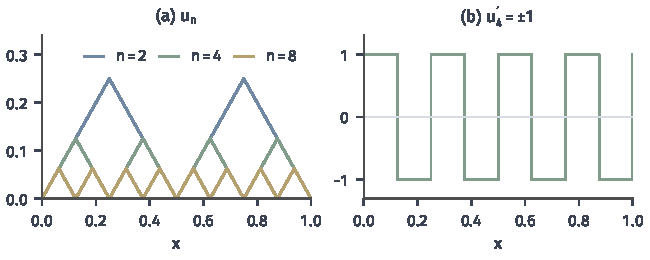
\includegraphics[width=110mm]{figures/03-optimization-evolution-and-signals/01-optimization/matplotlib/c9-bolza-sawtooth/figure.pdf}
  \caption{取不到下确界的最小化序列。(a)~斜率为$\pm1$、齿高$1/(2n)$的锯齿$u_n$，$n=2,4,8$，在$J(u)=\int_0^1((u'^2-1)^2+u^2)\,dx$下$J(u_n)=1/(12n^2)$；(b)~$u_4'$在$\pm1$间交替。$u_n$一致趋于零，$u_n'$弱收敛到零但$|u_n'|$恒为$1$，弱极限$0$的目标值为$1$。}
  \label{fig:opt-fn-bolza-sawtooth}
\end{figure}

两个例子中的目标都连续，下水平集也有界，可见目标连续不足以单独保证达到下确界。缺失的是目标在弱极限下的行为：能量可以藏进振荡或越来越远的坐标中，在弱极限里消失，而目标并不因此变小。

\paragraph{需要逐项检查的三件事}
按极限论证的步骤，问题分成三个。第一，最小化序列能否保持有界；第二，能否从中选出某种意义下收敛的子列；第三，极限是否仍可行，且目标值不超过序列目标值的下极限。第二步在Hilbert空间中由卷二已证明的结论提供：Hilbert空间中的每个有界序列都有弱收敛的子列，即存在$u$使$\langle w,u_{n_k}\rangle\to\langle w,u\rangle$对每个$w$成立，记作$u_{n_k}\rightharpoonup u$。同一处还证明了范数在弱极限下只能下降：$u_n\rightharpoonup u$推出$\|u\|\le\liminf_n\|u_n\|$。第一、三步则必须针对具体目标与约束检查。驻点方程有形式解，并不能反推出这些条件成立。

\subsection{直接法}
\label{sec:opt-fn-direct-method}

把三件事写成可以检查的条件，就得到下面的存在性定理。先给出两个与弱收敛配套的概念：若$u_n\in C$、$u_n\rightharpoonup u$总推出$u\in C$，称$C$\term{弱序列闭}（weakly sequentially closed）；若$u_n\rightharpoonup u$（均在$C$中）总推出$J(u)\le\liminf_nJ(u_n)$，称$J$在$C$上\term{弱序列下半连续}（weakly sequentially lower semicontinuous）。

\begin{theorem}[直接法]
\label{thm:opt-fn-direct-method}
设$H$为实Hilbert空间，$C\subseteq H$非空且弱序列闭，$J:H\to\mathbb R\cup\{+\infty\}$满足：
\begin{enumerate}
 \item 存在$u_0\in C$使$J(u_0)<+\infty$；
 \item 下水平集$S=\{u\in C:J(u)\le J(u_0)\}$有界；
 \item $J$在$C$上弱序列下半连续。
\end{enumerate}
则$J$在$C$上的下确界有限，并在某个$u^\star\in C$处达到。
\end{theorem}

\begin{proof}
记$m=\inf_CJ$，$m\le J(u_0)<+\infty$，暂不排除$m=-\infty$。

第一步，有界的最小化序列。取$u_n\in C$使$J(u_n)\to m$；去掉开头有限项后可设$J(u_n)\le J(u_0)$，于是$u_n\in S$，由条件2，$(u_n)$有界。

第二步，弱收敛子列。由Hilbert空间中有界序列的弱子列定理，存在子列$u_{n_k}\rightharpoonup u^\star$。

第三步，极限可行。$C$弱序列闭，所以$u^\star\in C$。

第四步，下极限比较。由条件3，$J(u^\star)\le\liminf_kJ(u_{n_k})=m$。$J$不取$-\infty$，所以$m>-\infty$；又$u^\star\in C$，$J(u^\star)\ge m$，故$J(u^\star)=m$。
\end{proof}

证明中“目标有下界”不是额外的假设，而是第四步的结论。条件2常由\term{强制性}（coercivity）得到：若$\|u\|\to\infty$（$u\in C$）时$J(u)\to+\infty$，则任何下水平集都有界。直接法只回答存在，不回答唯一。

\paragraph{唯一性另需凸性}
若$C$凸，$J$在$C$上严格凸，即$u\neq v$、$t\in(0,1)$时$J(tu+(1-t)v)<tJ(u)+(1-t)J(v)$，则最小点至多一个：设$u_1\neq u_2$都达到$m$，中点在$C$中且$J\bigl(\frac{u_1+u_2}2\bigr)<m$，矛盾。存在与唯一是两个独立的结论，分别由直接法与严格凸性提供。

\paragraph{如何检查弱序列闭与弱下半连续}
以下几条在例子中最常用。若$B:H\to Y$是到另一个Hilbert空间的有界线性算子，则$u_n\rightharpoonup u$推出$Bu_n\rightharpoonup Bu$，因为对每个$w\in Y$，$u\mapsto\langle w,Bu\rangle_Y$是$H$上的有界线性泛函。结合范数的弱下半连续性，$\frac12\|Bu-y\|_Y^2$在$H$上弱序列下半连续。由有限个有界线性泛函的等式或不等式$L_iu=c_i$、$L_iu\le c_i$定义的集合弱序列闭，因为弱收敛下每个$L_iu_n\to L_iu$。一般的闭凸集与凸下半连续目标同样满足这两条性质，这要用到下一小节的投影，届时再证明。

\paragraph{反面：非凸目标}
上一小节的两个例子都满足条件1与条件2，失败在条件3：$(\|\bm x\|_2^2-1)^2$与$(u'^2-1)^2$对$\bm x$或$u'$不凸，弱极限可以抬高它们的值。这说明一般非凸目标的范数连续性或范数下半连续性，都不能代替弱下半连续性。

\paragraph{反射空间（补充）}
证明中只有第二步用到Hilbert结构。卷二还证明了反射Banach空间中有界序列有弱收敛子列；$1<p<\infty$时$L^p$与$W^{1,p}$都是反射空间。在这样的空间中，把三个条件中的弱收敛按对偶空间理解，同样的四步证明照样成立。

\paragraph{导数平方能量满足全部条件}
回到章首的问题：$H=H^1(0,1)$，$C=\{u:u(0)=0,u(1)=1\}$，$J_0(u)=\frac12\|u'\|_{L^2}^2$。一维$H^1$中点值是有界线性泛函，所以$C$弱序列闭；$u\mapsto u'$是$H^1\to L^2$的有界线性算子，所以$J_0$弱序列下半连续。对$u\in C$，$|u(x)|=|\int_0^xu'\,dt|\le\|u'\|_{L^2}$，于是$\|u\|_{L^2}^2\le\|u'\|_{L^2}^2$，
\[
 \|u\|_{H^1}^2=\|u\|_{L^2}^2+\|u'\|_{L^2}^2\le4J_0(u) ,
\]
下水平集有界。直接法给出最小点存在，与第~\ref{sec:opt-fn-euler-lagrange}节直接验证的结果一致。高维区域上，起同样作用的是Poincaré不等式：在$H_0^1(\Omega)$中$\|u\|_{L^2}\le C_\Omega\|\nabla u\|_{L^2}$，因此固定边界迹时导数平方能量控制整个$H^1$范数。

\paragraph{线性增长的能量}
对第~\ref{sec:opt-fn-first-variation}节的平滑导数幅度~\eqref{eq:opt-fn-smoothed-tv}，情况不同。一维固定端点时，令$u_\delta$在$[\frac12-\frac\delta2,\frac12+\frac\delta2]$上从$0$线性升到$1$，其余位置为常数。它属于$C$，并且
\[
 \int_0^1|u_\delta'|\,dx=1,\qquad\int_0^1|u_\delta'|^2dx=\frac1\delta ,\qquad J_\varepsilon(u_\delta)\le\int_0^1(|u_\delta'|+\varepsilon)\,dx=1+\varepsilon .
\]
$\delta\to0$时$\|u_\delta\|_{H^1}\to\infty$，而目标值保持有界：下水平集在$H^1$中无界，条件2不成立（图~\ref{fig:opt-fn-transition-width}）。原因是$\psi_\varepsilon(p)$只随$|p|$线性增长，无法像平方那样惩罚越来越陡的过渡。检查失败并不证明最小点不存在：这个一维问题中，$\psi_\varepsilon$凸，由Jensen不等式$J_\varepsilon(u)\ge\psi_\varepsilon\bigl(\int_0^1u'\,dx\bigr)=\sqrt{1+\varepsilon^2}=J_\varepsilon(x)$，直线仍是最小点。但在一般问题中，陡峭过渡的极限是跳跃，它已不在$H^1$中。允许跳跃需要换到有界变差函数等新空间，附加平方增长项则改变了目标；两种处理都须重新核验条件，本书不展开有界变差空间的存在理论。

\begin{figure}[!htb]
  \centering
  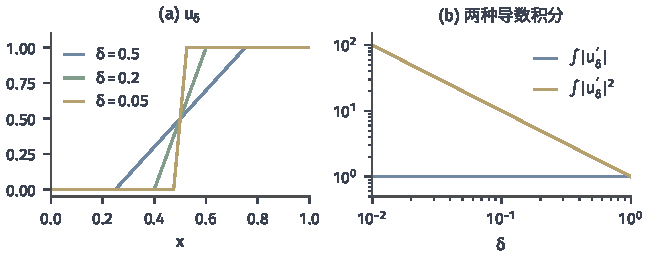
\includegraphics[width=110mm]{figures/03-optimization-evolution-and-signals/01-optimization/matplotlib/c9-transition-width/figure.pdf}
  \caption{宽度为$\delta$的单位过渡。(a)~在$x=1/2$附近宽$\delta=0.5,0.2,0.05$的区间内从$0$线性升到$1$的$u_\delta$；(b)~导数幅度积分$\int|u_\delta'|$恒为$1$（蓝），导数平方积分$\int|u_\delta'|^2=1/\delta$随$\delta\to0$增长（黄），两轴均为对数。线性增长的能量不能阻止过渡变陡。}
  \label{fig:opt-fn-transition-width}
\end{figure}

\subsection{闭凸集投影}
\label{sec:opt-fn-projection}

第~\ref{chap:opt-nonsmooth}章把有限维闭凸集上的投影作为邻近映射的特例建立起来，第~\ref{chap:constrained-optimization}章用它构造约束迭代。在一般Hilbert空间中，“离给定元素最近的可行点”同样是一个泛函最小化问题。它的结构足够好，可以不借直接法，只用完备性和平行四边形恒等式完整证明存在唯一。

\begin{theorem}[闭凸集上的投影]
\label{thm:opt-fn-projection}
设$H$为实Hilbert空间，$C\subseteq H$非空、闭且凸，$z\in H$。则存在唯一的$p\in C$使
\[
 \|z-p\|_H=\inf_{u\in C}\|z-u\|_H .
\]
记$p=\Pi_Cz$，称为$z$在$C$上的\term{投影}（projection）。
\end{theorem}

\begin{proof}
记$d=\inf_{u\in C}\|z-u\|_H$，取$u_n\in C$使$\|z-u_n\|_H\to d$。

第一步，最小化序列是Cauchy列。对$z-u_n$与$z-u_k$用平行四边形恒等式，
\[
 \|u_n-u_k\|_H^2=2\|z-u_n\|_H^2+2\|z-u_k\|_H^2-4\Bigl\|z-\frac{u_n+u_k}2\Bigr\|_H^2 .
\]
$C$凸，中点$\frac{u_n+u_k}2\in C$，所以最后一项的范数平方至少为$d^2$。于是$\|u_n-u_k\|_H^2\le2\|z-u_n\|_H^2+2\|z-u_k\|_H^2-4d^2\to0$。

第二步，极限可行。$H$完备，$u_n$收敛到某个$p$；$C$闭，$p\in C$；由范数连续，$\|z-p\|_H=d$。

第三步，唯一。若$p_1,p_2\in C$都达到$d$，对它们用同一个恒等式，$\|p_1-p_2\|_H^2\le2d^2+2d^2-4d^2=0$。
\end{proof}

凸性在证明中出现了两次：中点留在$C$中，既让最小化序列成为Cauchy列，又排除了两个不同的最近点。完备性与闭性则保证极限存在且可行。闭线性子空间上的正交投影有同样结构的证明，见\BookChapterRef{chap:function-spaces}{卷二“函数空间”章}；那里中点留在子空间中，这里改用凸性保证同一件事。

\paragraph{钝角刻画}
投影点满足一个只涉及内积的条件，它是变分不等式~\eqref{eq:opt-fn-variational-inequality}的特例。

\begin{theorem}[投影的变分刻画]
\label{thm:opt-fn-projection-characterization}
在定理~\ref{thm:opt-fn-projection}的条件下，$p\in C$等于$\Pi_Cz$，当且仅当
\begin{equation}
 \langle z-p,u-p\rangle_H\le0\qquad\text{对所有}u\in C .
 \label{eq:opt-fn-projection-vi}
\end{equation}
\end{theorem}

\begin{proof}
必要性：$J(u)=\frac12\|z-u\|_H^2$在$H$上Fréchet可微，$DJ(p)[h]=\langle p-z,h\rangle_H$，由定理~\ref{thm:opt-fn-variational-inequality}(1)，$\langle p-z,u-p\rangle_H\ge0$，即~\eqref{eq:opt-fn-projection-vi}。充分性：对$u\in C$展开
\[
 \|z-u\|_H^2=\|z-p\|_H^2-2\langle z-p,u-p\rangle_H+\|u-p\|_H^2\ge\|z-p\|_H^2 .
\]
\end{proof}

几何上，~\eqref{eq:opt-fn-projection-vi}说$z-p$与从$p$指向$C$中任一点的向量夹角不小于直角（图~\ref{fig:opt-fn-projection-geometry}(a)）。若$C$是闭线性子空间$M$，取$u=p\pm w$（$w\in M$），两个不等式合起来给出$\langle z-p,w\rangle_H=0$：钝角条件加强为正交条件（图~\ref{fig:opt-fn-projection-geometry}(b)），回到卷二的正交投影。

\begin{figure}[!htb]
  \centering
  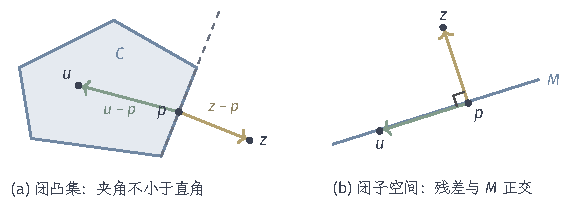
\includegraphics[width=96.725mm]{figures/03-optimization-evolution-and-signals/01-optimization/tikz/c9-projection-geometry/figure.pdf}
  \caption{Hilbert空间中投影的几何（平面示意）。(a)~闭凸集$C$（浅蓝）外一点$z$的投影$p$：残差$z-p$（黄）与任一$u-p$（绿）的夹角不小于直角，虚线为过$p$且与$z-p$垂直的支撑线；(b)~闭子空间$M$上，$u$可沿$M$向两侧取，钝角条件变为残差$z-p$与$M$正交。}
  \label{fig:opt-fn-projection-geometry}
\end{figure}

\paragraph{非扩张性}
对$z_1,z_2\in H$，记$p_i=\Pi_Cz_i$。在~\eqref{eq:opt-fn-projection-vi}中分别取$(z,p,u)=(z_1,p_1,p_2)$与$(z_2,p_2,p_1)$，两式相加得$\langle(z_1-z_2)-(p_1-p_2),p_2-p_1\rangle_H\le0$，即
\[
 \|p_1-p_2\|_H^2\le\langle z_1-z_2,p_1-p_2\rangle_H\le\|z_1-z_2\|_H\|p_1-p_2\|_H .
\]
所以$\|\Pi_Cz_1-\Pi_Cz_2\|_H\le\|z_1-z_2\|_H$：投影不放大距离，称为非扩张。这与有限维中的性质相同，证明也只用了内积。

\paragraph{闭凸集弱序列闭}
钝角刻画回答了上一小节留下的问题。设$C$非空闭凸，$u_n\in C$，$u_n\rightharpoonup u$。令$p=\Pi_Cu$，由~\eqref{eq:opt-fn-projection-vi}，$\langle u-p,u_n-p\rangle_H\le0$对每个$n$成立；令$n\to\infty$，由弱收敛得$\langle u-p,u-p\rangle_H\le0$，所以$u=p\in C$。进一步，若$J$凸且（按范数）下半连续，则每个下水平集$\{J\le c\}$闭且凸，因而弱序列闭。设$u_n\rightharpoonup u$而$J(u)>\liminf_nJ(u_n)$，取$c$严格介于两者之间，则有子列始终落在$\{J\le c\}$中，其弱极限$u$也在其中，$J(u)\le c$，矛盾。所以凸且下半连续的目标弱序列下半连续，直接法的条件3对它自动成立。

\paragraph{检查候选集}
均值约束$C=\{u\in L^2(0,1):\int_0^1u\,dx=1\}$是有界线性泛函$u\mapsto\int_0^1u$的一个水平集，闭且凸。它的投影是$\Pi_Cz=z+(1-\int_0^1z)\cdot\mathbf 1$：残差$z-\Pi_Cz$为常数，与$C$中任意两元之差（均值为零）正交，满足~\eqref{eq:opt-fn-projection-vi}且等号成立。例如$z(x)=x$时$\Pi_Cz=x+\frac12$。点值约束则要小心：在$L^2(0,1)$的等价类上，“$u(1/2)=0$”没有意义，因为改变一个零测集上的值不改变元素；只有在点值是连续线性泛函的空间中（如一维$H^1$）才能用这样的约束定义闭凸集。

\paragraph{凸性与闭性不能省}
非凸集合可能有多个最近点：在单位球面$\{\|u\|_H=1\}$上，零元到每一点的距离都是$1$。也可能一个都没有：在$\ell^2$中取$C=\{(1+\frac1k)\bm e_k:k\ge1\}$，任两点距离大于$\sqrt2$，所以$C$闭；零元到$C$的距离下确界为$1$，却没有哪一点距离恰为$1$。有限维中的投影算法因此不能不加条件地当成无限维的求解保证：可行集的闭性与凸性都要先在所选空间中核实。

% 第9章第5节：泛函优化的有限维近似（试探空间与Ritz方法、离散目标的构造、误差来源）。

\section{泛函优化的有限维近似}
\label{sec:opt-fn-approximation}

计算机只能处理有限个数。要把泛函优化交给前面各章的算法，必须把候选函数和目标都化成有限维对象。本节分开说明两种化法：限制候选的表示，以及改造目标的计算公式；最后把由此产生的误差按来源区分，因为“算出来的数”同时受到这几种近似的影响。

\subsection{试探空间与Ritz方法}
\label{sec:opt-fn-ritz}

最直接的办法是只在有限个函数张成的集合里找候选。目标的定义保持不变，只是把搜索范围缩小。

\paragraph{有限表示与系数导数}
选择满足必要边界条件的试探函数，写
\[
 u_{\bm a}=u_0+\sum_{j=1}^Na_j\varphi_j,\qquad\bm a\in\mathbb R^N ,
\]
其中$u_0$实现规定的边界值，每个$\varphi_j$的边界值为零，于是每个$u_{\bm a}$都满足本质边界条件。$\varphi_1,\dots,\varphi_N$张成的空间称为\term{试探空间}（trial space）。把泛函限制在这一族上，得到有限维目标$J_N(\bm a)=J(u_{\bm a})$，在其上求最小，这就是\term{Ritz方法}（Ritz method）。映射$\bm a\mapsto u_{\bm a}$是仿射的，由链式法则（定理~\ref{thm:opt-fn-chain-rule}），只要$J$在$u_{\bm a}$处Fréchet可微，
\begin{equation}
 \frac{\partial J_N}{\partial a_j}(\bm a)=DJ(u_{\bm a})[\varphi_j],\qquad j=1,\dots,N .
 \label{eq:opt-fn-ritz-gradient}
\end{equation}
有了~\eqref{eq:opt-fn-ritz-gradient}，就可以调用第~\ref{chap:opt-smooth}章的梯度型或Newton型方法，或在二次目标时直接解线性方程组。

\begin{example}[帽函数上的Ritz方法]
\label{ex:opt-fn-ritz-hat}
在$[0,1]$上最小化$J(u)=\int_0^1\bigl(\frac12u'^2-fu\bigr)\,dx$，$u(0)=u(1)=0$，取$f(x)=\pi^2\sin(\pi x)$。内部方程是$-u''=f$，满足边界条件的解为$u^\star(x)=\sin(\pi x)$；目标凸，与第~\ref{sec:opt-fn-euler-lagrange}节相同的平方差展开说明它是唯一最小点。把区间等分为$N$段，节点$x_j=j\Delta x$，$\Delta x=1/N$，取帽函数
\[
 \varphi_j(x)=\max\Bigl(0,\ 1-\frac{|x-x_j|}{\Delta x}\Bigr),\qquad j=1,\dots,N-1 .
\]
$\varphi_j$在$x_j$处为$1$，在其他节点为$0$，所以系数$a_j$就是$u_{\bm a}$在节点$x_j$处的值；$u_0=0$。代入目标，
\[
 J_N(\bm a)=\frac12\bm a^\top\bm K\bm a-\bm b^\top\bm a,\qquad K_{i,j}=\int_0^1\varphi_i'\varphi_j'\,dx,\quad b_j=\int_0^1f\varphi_j\,dx .
\]
$\varphi_j'$在$x_j$左侧为$1/\Delta x$、右侧为$-1/\Delta x$，于是$\bm K$是对角元$2/\Delta x$、相邻非对角元$-1/\Delta x$的三对角矩阵，对称正定，最小点由$\bm K\bm a=\bm b$唯一确定。

图~\ref{fig:opt-fn-ritz-hat}(a)画出$N=4$与$N=8$的结果：折线的节点值与$\sin(\pi x)$重合。这是本例的特殊性质：由$-u^{\star\prime\prime}=f$分部积分，$b_j=\int_0^1u^{\star\prime}\varphi_j'\,dx=\bigl(2u^\star(x_j)-u^\star(x_{j-1})-u^\star(x_{j+1})\bigr)/\Delta x$，恰好是$\bm K$作用在节点值向量上的第$j$个分量，所以$a_j=u^\star(x_j)$。(b)中，网格每加密一倍，导数误差$\|(u^\star-u_N)'\|_{L^2}$约减半（$N=4,8,16$时约为$0.499$、$0.251$、$0.126$），函数值误差$\|u^\star-u_N\|_{L^2}$约降为四分之一。这是对本例的数值观察；一般条件下离散解收敛的证明属于第~\ref{part:dynamical-systems-control-and-decision}部分。
\end{example}

\begin{figure}[!htb]
  \centering
  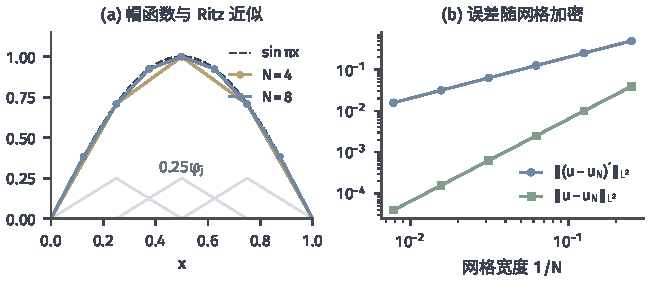
\includegraphics[width=110mm]{figures/03-optimization-evolution-and-signals/01-optimization/matplotlib/c9-ritz-hat/figure.pdf}
  \caption{帽函数试探空间上的Ritz方法，问题为$\min\int_0^1(\frac12u'^2-\pi^2\sin(\pi x)\,u)\,dx$，$u(0)=u(1)=0$，精确解$\sin(\pi x)$（黑色虚线）。(a)~$N=4$时的三个帽函数（灰，缩小为$0.25$倍）及$N=4$（黄）、$N=8$（蓝）的分段线性近似；(b)~$N=4,8,\dots,128$时导数误差（蓝）与函数值误差（绿）随网格宽度的变化，双对数坐标，斜率约为$1$与$2$。误差积分用每段6点Gauss--Legendre求积。}
  \label{fig:opt-fn-ritz-hat}
\end{figure}

\paragraph{改变的是候选集合}
Ritz方法把可行集$C$换成了$C\cap(u_0+\operatorname{span}\{\varphi_j\})$，目标本身没有改变，积分也还没有近似：上例中$\bm K$和$\bm b$都是精确积分。因为可行集变小，$J_N$的最小值不低于原问题的最小值，二者之差就是试探空间的限制误差。返回的函数$u_{\bm a}$需要回到原问题核对约束：本质边界条件由构造保证，其他约束（如非负性）则要另行检查。有限维问题本身是否有解，也须按$J_N$的目标与约束重新判断；上例靠的是$\bm K$正定。

\paragraph{系数梯度与函数梯度}
\eqref{eq:opt-fn-ritz-gradient}给出的是对系数的偏导数，它和按函数内积定义的梯度不同。若要在试探空间中找$L^2$梯度$g=\sum_jc_j\varphi_j$，条件$\langle g,\varphi_i\rangle_{L^2}=DJ(u_{\bm a})[\varphi_i]$写成
\[
 \bm M\bm c=\nabla_{\bm a}J_N(\bm a),\qquad M_{i,j}=\langle\varphi_i,\varphi_j\rangle_{L^2} .
\]
$\bm M$是试探函数的Gram矩阵，在有限元语境中称为\term{质量矩阵}（mass matrix）。帽函数两两不正交，等距网格上$\bm M$是对角元$2\Delta x/3$、相邻非对角元$\Delta x/6$的三对角矩阵。只有基函数关于所用内积标准正交时，$\bm M$才是单位矩阵，系数梯度才等于函数梯度的系数。

\subsection{离散目标的构造}
\label{sec:opt-fn-discrete-objective}

另一种化法不先选试探函数，而是直接把目标中的导数和积分换成有限的差分与求和。这样得到的是一个新的目标，需要单独说明它与原目标的关系。

\paragraph{差分与求和}
从一维导数平方能量$\frac12\int_0^1|u'|^2dx$出发，把区间等分为$N$段，网格宽度$\Delta x=1/N$，节点$x_i=i\Delta x$。在第$i$段上用差商$(u_{i+1}-u_i)/\Delta x$近似导数，再乘以积分单元的长度$\Delta x$，得到
\begin{equation}
 E_N(u)=\frac12\sum_{i=0}^{N-1}\Bigl(\frac{u_{i+1}-u_i}{\Delta x}\Bigr)^2\Delta x=\sum_{i=0}^{N-1}\frac{(u_{i+1}-u_i)^2}{2\Delta x} .
 \label{eq:opt-fn-discrete-energy}
\end{equation}
同一个公式有两种用途。一是固定一个已知函数$u$，取$u_i=u(x_i)$，用$E_N(u)$近似它的能量值；二是把节点值$(u_0,\dots,u_N)$本身当作未知量，在其上优化。后者若再固定$u_0,u_N$，就与上一小节的帽函数Ritz方法重合：分段线性函数在每段上导数恒为差商，$E_N$恰好等于$\frac12\int|u'|^2$。网格不等距时分母要换成各段的宽度；积分权重、边界处理一旦改变，$E_N$就是另一个目标，须重新核算。

\paragraph{点云上的图能量}
没有规则网格时，只有一组点$x_1,\dots,x_n$及其上的取值$u_i$。给定对称非负权重$w_{i,j}=w_{j,i}$，例如由点间距离经核函数算出，定义
\begin{equation}
 E_w(u)=\frac14\sum_{i=1}^n\sum_{j=1}^nw_{i,j}(u_i-u_j)^2=\frac12\sum_{\{i,j\}}w_{i,j}(u_i-u_j)^2 .
 \label{eq:opt-fn-graph-energy}
\end{equation}
左式对有序点对求和，每条无向边被计了两次，所以系数为$\frac14$；右式每条无向边只计一次，系数为$\frac12$，二者相等。写成矩阵，$E_w(u)=\frac12\bm u^\top\bm L\bm u$，其中$\bm L=\bm D-\bm W$，$\bm D$是以$D_{i,i}=\sum_jw_{i,j}$为对角元的对角矩阵。例如三点上$w_{1,2}=1$、$w_{2,3}=2$、$w_{1,3}=0$，取$\bm u=(0,1,3)$，右式给出$\frac12(1\cdot1^2+2\cdot2^2)=4.5$，左式给出$\frac14(2\cdot1+2\cdot8)=4.5$。若要把$E_w$解释为某个连续能量的近似，还需另外给定采样密度、邻近尺度、核权重与样本数的归一化；这些条件不全时，结论只属于图上的离散目标。点云位于曲面上时的几何比较涉及流形，可参考\BookChapterRef{chap:differential-geometry-and-symmetry}{卷四“非线性空间与流形”章}。

\paragraph{改目标与换内积}
回到第~\ref{sec:opt-fn-hilbert-gradient}节的区分。改变网格权重或边权$w_{i,j}$，改变的是目标本身，最小点一般随之改变。固定目标，改用另一个内积计算梯度（例如用$\bm M$或$\bm L+\bm I$代替单位矩阵），改变的是梯度的表示和迭代轨迹，不改变最小点。两种操作在离散公式中都表现为“乘一个矩阵权重”，形式相似，但不能用换内积去补偿一个未经论证的目标离散。

\subsection{误差来源}
\label{sec:opt-fn-error-sources}

一次数值计算交出的结果，同时受三种近似影响：试探空间限制了候选，离散公式改变了目标，有限次迭代没有精确求出离散问题的最小点。比较它们时，每次只改变一个环节，其余固定。

\paragraph{固定函数的能量一致性}
先只看目标离散。下面的结论比较的是同一个已知函数的两个能量值，与优化无关。

\begin{theorem}[差分能量的一致性]
\label{thm:opt-fn-energy-consistency}
设$u\in C^1[0,1]$，$u_i=u(x_i)$，则$N\to\infty$时$E_N(u)\to\frac12\int_0^1u'(x)^2\,dx$。
\end{theorem}

\begin{proof}
由中值定理，每段上存在$\xi_i\in(x_i,x_{i+1})$使$(u_{i+1}-u_i)/\Delta x=u'(\xi_i)$，所以$E_N(u)=\frac12\sum_iu'(\xi_i)^2\Delta x$。这是连续函数$u'^2$在$[0,1]$上的一个Riemann和。$u'^2$在闭区间上一致连续：对任意$\varepsilon>0$，当$\Delta x$足够小时，同一段内任两点处$u'^2$之差小于$\varepsilon$，于是Riemann和与积分之差不超过$\varepsilon$。
\end{proof}

取$u=\sin(\pi x)$可以算出精确值。由$\sin\alpha-\sin\beta=2\cos\frac{\alpha+\beta}2\sin\frac{\alpha-\beta}2$及$\sum_{i=0}^{N-1}\cos^2\bigl(\pi(i+\frac12)/N\bigr)=N/2$（$N\ge2$），
\[
 E_N(\sin\pi x)=N^2\sin^2\frac\pi{2N}=\frac{\pi^2}4-\frac{\pi^4}{48N^2}+O(N^{-4}) .
\]
图~\ref{fig:opt-fn-energy-consistency}显示，$N=2$时$E_N=2$，$N=8$时约为$2.436$，误差随$N^{-2}$下降。定理只说明固定函数的能量值收敛，它还没有比较两个优化问题的最小点：离散最小点是否收敛到连续最小点，需要另外的稳定性与逼近条件。

\begin{figure}[!htb]
  \centering
  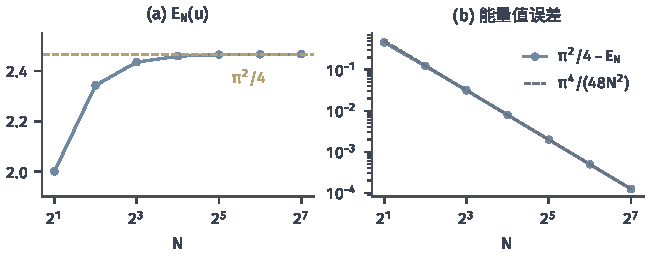
\includegraphics[width=110mm]{figures/03-optimization-evolution-and-signals/01-optimization/matplotlib/c9-energy-consistency/figure.pdf}
  \caption{固定函数$u=\sin(\pi x)$的差分能量~\eqref{eq:opt-fn-discrete-energy}。(a)~$E_N(u)=N^2\sin^2(\pi/(2N))$随$N=2,4,\dots,128$趋于$\pi^2/4\approx2.467$（黄色虚线）；(b)~误差$\pi^2/4-E_N$（蓝）与渐近式$\pi^4/(48N^2)$（灰色虚线）几乎重合，双对数坐标。}
  \label{fig:opt-fn-energy-consistency}
\end{figure}

\paragraph{边权扰动的目标值界}
对点云上的固定记录$\bm u$，同一计数口径下只改变边权，从$w$换成$\widetilde w$。逐项相减，
\[
 \bigl|E_w(u)-E_{\widetilde w}(u)\bigr|\le\frac14\sum_{i,j}|w_{i,j}-\widetilde w_{i,j}|(u_i-u_j)^2 .
\]
上面的三点例子中，把$w_{1,2}$从$1$改为$1.1$（$w_{2,1}$随之改变），右边为$\frac14\cdot2\cdot0.1\cdot1=0.05$，而$E_{\widetilde w}(u)=4.55$，差恰为$0.05$。这个界是同一记录上的目标值扰动界。若两个目标各自重新优化，最小点之间相差多少还依赖强制性、唯一性或其他稳定性条件，不能从这个不等式直接读出。

\paragraph{报告数值结果时}
迭代停止时，宜把三件事分开核验：离散目标是否已充分下降（例如梯度范数或对偶间隙）；返回的函数是否保留了原问题的约束；所用离散目标是否在相关函数上一致地近似连续目标。能量值的一致性、连续最小点的存在、离散最小点的收敛与求解器的收敛是四个不同的命题。本章分别给出了第一个的简单情形与第二个的直接法；具体方程的网格解收敛，由第~\ref{part:dynamical-systems-control-and-decision}部分在相应的一致性、稳定性与逼近条件下建立。

% 第9章第6节：本章小结。

\section{本章小结}
\label{sec:opt-fn-summary}

章首问：连接$(0,0)$与$(1,1)$、使$\frac12\int_0^1u'^2dx$最小的曲线是哪一条，这个问题该怎样提、怎样解。现在可以按步骤回答。先明确候选空间与目标：取$X=H^1(0,1)$，能量在整个空间上有限，端点条件写进可行集$C$。再用微分计算小扰动的响应：方向导数是沿一条直线的一元导数，Gâteaux微分要求这些响应组成有界线性泛函，Fréchet微分进一步要求余项对所有小扰动统一地小；Hilbert空间中，微分借内积写成梯度，而梯度随内积改变。

最优条件按允许的扰动方向写出。无约束或仿射约束下微分在方向空间上为零，凸约束下变为变分不等式；这些都是必要条件，充分性来自凸性，或来自具有一致下界的二阶项。积分目标经分部积分分成内部与边界两部分：测试函数给出Euler--Lagrange方程或其弱形式，自由边界给出自然边界条件，固定边界则作为本质条件写进可行集。对章首问题，方程给出候选$u=x$，平方差展开证明它是唯一最小点。

这些条件都不负责存在性。最小化序列可以在函数值趋于下确界的同时振荡或逃逸，极限取不到最小值；直接法用有界性、弱收敛子列、弱序列闭性和弱下半连续性逐步排除这些情形，闭凸集投影则只用完备性与平行四边形恒等式给出存在唯一。最后，有限维近似或者改变候选集合（Ritz方法），或者改变目标（差分与图能量），二者都需要独立检查误差；固定函数的能量一致性不等于离散最小点收敛。表~\ref{tab:opt-fn-summary}汇总了本章各结论的条件与边界。具体的函数拟合由上一章主讲，时间演化、梯度流与方程解理论由第~\ref{part:dynamical-systems-control-and-decision}部分接续。

\begin{table}[!htb]
  \centering
  \small
  \begin{tabularx}{\linewidth}{@{}l>{\raggedright\arraybackslash}X>{\raggedright\arraybackslash}X@{}}
    \toprule
    问题 & 本章的工具与结论 & 所需条件与边界 \\
    \midrule
    小扰动的响应 & 方向导数、Gâteaux微分、Fréchet微分；Hilbert梯度 & 目标在点的开邻域内有限；Fréchet余项依赖所选范数；梯度依赖内积 \\
    候选是否最优 & 一阶条件、变分不等式、二阶条件 & 以最小点存在为前提；充分性需凸性或一致正定的二阶项 \\
    积分目标的条件 & Euler--Lagrange方程（弱形式）、自然边界条件 & 交换极限与积分需支配条件；点态方程需额外正则性 \\
    最小值是否达到 & 直接法；闭凸集投影存在唯一 & 下水平集有界、弱序列闭、弱下半连续；唯一性另需严格凸 \\
    怎样计算 & Ritz方法、差分能量、图能量 & 改变候选集合或目标；能量一致性不等于最小点收敛 \\
    \bottomrule
  \end{tabularx}
  \caption{泛函优化各环节的工具与条件。}
  \label{tab:opt-fn-summary}
\end{table}

